\documentclass{article}
\usepackage[italian]{babel}
\usepackage[T1]{fontenc}
\usepackage[utf8]{inputenc}
\usepackage{hyperref}
\usepackage{graphicx}
\usepackage{caption}
\usepackage{pgfplots}
\usepackage{tikz}
\usepackage{filecontents}
\usepackage{amsmath}
\usepackage{amsfonts}
\usepackage{amssymb}
\usepackage{gensymb}
\usepackage{cancel}
\usepackage{xcolor}
\usepackage{textcomp}
\usepackage{booktabs}

\pgfplotsset{compat=1.9}

\def\mathunderline#1#2{\color{#1}\underline{{\color{black}#2}}\color{black}}

\newcommand{\Laplace}{\mathop{\mathcal{L}}}
\newcommand{\AntiLaplace}{\mathop{\mathcal{L}^{-1}}}
\newcommand{\Fourier}{\mathop{\mathcal{F}}}
\newcommand{\AntiFourier}{\mathop{\mathcal{F}^{-1}}}
\newcommand{\Ztransf}{\mathop{\mathcal{Z}}}
\newcommand{\AntiZtransf}{\mathop{\mathcal{Z}^{-1}}}

\hypersetup{hidelinks}

\begin{filecontents} {discrete.dat}
	 n		 xn
   -5.0		-5.0
   -4.0		-4.0
   -3.0		-3.0
   -2.0		-2.0
   -1.0		-1.0
    0.0		 0.0
    1.0		 1.0
    2.0		 2.0
    3.0		 3.0
    4.0		 4.0
    5.0		 5.0
\end{filecontents}

\begin{filecontents} {discrete_pulse.dat}
	  n		 xn
	-5.0	 0.0
	-4.0	 0.0
	-3.0	 0.0
	-2.0	 0.0
	-1.0	 0.0
 	 0.0	 1.0
 	 1.0	 0.0
 	 2.0	 0.0
 	 3.0	 0.0
 	 4.0	 0.0
 	 5.0	 0.0
\end{filecontents}

\begin{filecontents} {discrete_signal_ex.dat}
	  n		 xn
	-4.0	-2.0
	-3.0	 3.0
	-2.0	 3.0
	-1.0	-2.0
 	 0.0	 4.0
 	 1.0	 2.0
 	 2.0	-4.0
 	 3.0	-2.0
 	 4.0	 1.0
\end{filecontents}

\begin{filecontents} {discrete_signal_pulse_1.dat}
	  n		 xn
	-5.0	0.0
	-4.0	0.0
	-3.0	0.0
	-2.0	3.0
	-1.0	0.0
 	 0.0	0.0
 	 1.0	0.0
 	 2.0	0.0
 	 3.0	0.0
 	 4.0	0.0
 	 5.0	0.0
\end{filecontents}

\begin{filecontents} {discrete_signal_pulse_2.dat}
	  n		 xn
	-5.0	 0.0
	-4.0	 0.0
	-3.0	 0.0
	-2.0	 0.0
	-1.0	-2.0
 	 0.0	 0.0
 	 1.0	 0.0
 	 2.0	 0.0
 	 3.0	 0.0
 	 4.0	 0.0
 	 5.0	 0.0
\end{filecontents}

\begin{filecontents} {discrete_signal_pulse_3.dat}
	  n		 xn
	-5.0	 0.0
	-4.0	 0.0
	-3.0	 0.0
	-2.0	 0.0
	-1.0	 0.0
 	 0.0	 4.0
 	 1.0	 0.0
 	 2.0	 0.0
 	 3.0	 0.0
 	 4.0	 0.0
 	 5.0	 0.0
\end{filecontents}

\begin{filecontents} {discrete_signal_pulse_4.dat}
	  n		 xn
	-5.0	 0.0
	-4.0	 0.0
	-3.0	 0.0
	-2.0	 0.0
	-1.0	 0.0
 	 0.0	 0.0
 	 1.0	 2.0
 	 2.0	 0.0
 	 3.0	 0.0
 	 4.0	 0.0
 	 5.0	 0.0
\end{filecontents}

\begin{filecontents} {discrete_signal_pulse_5.dat}
	  n		 xn
	-5.0	 0.0
	-4.0	 0.0
	-3.0	 0.0
	-2.0	 0.0
	-1.0	 0.0
 	 0.0	 0.0
 	 1.0	 0.0
 	 2.0	-4.0
 	 3.0	 0.0
 	 4.0	 0.0
 	 5.0	 0.0
\end{filecontents}

\begin{filecontents} {RdC_l1.dat}
	Re		Im
	-2		 4
\end{filecontents}

\begin{filecontents} {RdC_l2.dat}
	Re		Im
	-4		 2
\end{filecontents}

\pgfplotsset{compat=newest}

\begin{document}
    \clearpage

    \begin{titlepage}
       \centering
       \vspace*{\fill}
       {\scshape\LARGE Università degli Studi di Verona \par}
       \vspace{1.5cm}
       \line(1,0){145} \\
       {\huge\bfseries Sistemi\par}
       \line(1,0){145} \\
       \vspace{0.5cm}
       {\scshape\Large Appunti del corso\par}
       \vspace{2cm}
       {\Large\itshape Mattia Zorzan\par}
       \vspace{1cm}

       \vspace{5cm}
       \vspace*{\fill}
       % Bottom of the page
       {\large \today\par}
    \end{titlepage}
    \thispagestyle{empty}

    \tableofcontents

    \newpage

    \section{Introduzione}
        La presente è una dispesa \LaTeX contenente gli appunti per il corso di Sistemi. Alla presente potranno essere aggiunte integrazioni prese dal libro \textbf{Signals and Systems: Pearson New International Edition} di \textit{Alan V. Oppenheim} con lo scopo di integrare parti meno chiare del corso. \\
        Il codice \LaTeX è disponibile a:

        \begin{center}
            \url{https://github.com/davbianchi/dispense-info-univr}
        \end{center}

    \newpage

    \section{Definizoni}
        \textbf{Sistema} - Modello matematico che rappresenta un fenomeno che evolve nel tempo in modo deterministico. \\
        \textbf{Segnale} - Grandezza fisica variabile nel tempo, a cui è assegnata un'informazione. \\
        \\
        Lasciando perdere le definizioni, che vogliono dire tutto e niente in questo caso, ci si può ricondurre all'amata matematica per aiutarsi un pochino. Matematicamente i \textit{segnali} sono rappresentati come funzioni di una o più variabili indipendenti. La definizione di segnale usa il tempo come variabile indipendente, anche se se ne potrebbero utilizzare altre in casi diversi. \\
        \\
        Considereremo due tipi di segnali, \textit{continui} e \textit{discreti}. \\
        I segnali continui sono quelli in cui la variabile indipendente è rappresentata come un valore continuo, e questi sono definiti per un contnuum di valori della variabile indipendente. \\
        I segnali discreti sono definiti solo a tempo discreto (utlizzando il tempo come variabile indipendente) e di conseguenza sono definiti solo per un insieme discreto di valori della variabile indipendente. \\
        \\
        Il passaggio di uno stesso segnale da continuo a discreto avviene tramite un processo detto \textit{campionamento}. \\
		\\
		\textbf{N.B:} Si usa la notazione con le parentesi tonde per i segnali continui, quella con le parentesi quadre per i segnali discreti. La variabile indipendente è $ t $ per i segnali continui e $ n $ per quelli discreti.

		\begin{figure} [h]
			\begin{center}
				\begin{tikzpicture}% function
					\begin{axis} [
						axis lines=middle,
						xlabel={$ t $},
						ylabel={$ \boldsymbol{x(t)} $},
						xmin=-6, xmax=6,
						ymin=-6, ymax=6,
						xtick={-5, ..., 5},
						ytick={-5,..., 5},
						every axis x label/.style={
						    at={(ticklabel* cs:1.03)},
						    anchor=west,
						},
						every axis y label/.style={
						    at={(ticklabel* cs:1.03)},
						    anchor=south,
						},
					]
					\addplot [red, very thick, smooth] {x};
					\end{axis}
				\end{tikzpicture}
			\end{center}
			\captionsetup{labelformat=empty}
			\caption{\textit{Segnale continuo}}
		\end{figure}

		\begin{figure} [h]
			\begin{center}
				\begin{tikzpicture}% function
					\begin{axis} [
						axis lines=middle,
						xlabel={$n$},
						ylabel={$\boldsymbol{x[n]}$},
						xtick={-6, -5, ..., 6},
						ytick={-6, -5, ..., 6},
						xmin=-6, xmax=6,
						ymin=-6, ymax=6,
						xtick={-5, ..., 5},
						ytick={-5,..., 5},
						every axis x label/.style={
						    at={(ticklabel* cs:1.03)},
						    anchor=west,
						},
						every axis y label/.style={
						    at={(ticklabel* cs:1.03)},
						    anchor=south,
						},
					]
					\addplot [ycomb, red, very thick, mark=*] table [x={n}, y={xn}]  {discrete.dat};
					\end{axis}
				\end{tikzpicture}
			\end{center}
			\captionsetup{labelformat=empty}
			\caption{\textit{Segnale discreto}}
		\end{figure}

	\newpage

	\section{Tipi di Segnale}
		\subsection{Segnali Pari e Dispari}
			Un segnale $ x(t) $ o $ x[n] $ è \textit{pari} se è uguale alla sua controparte rovesciata, ovvero alla sua controparte ruotata di \textdegree{180} rispetto all'origine. \\
			Un segnale continuo è \textit{pari} se:
			\[
				x(-t)\; =\; x(t)
			\]
			Un segnale discreto è \textit{pari} se:
			\[
				x[-n]\; =\; x[n]
			\]
			Un segnale si dice \textit{dispari} se:
			\[
				\begin{aligned}
					&x(-t)\; =\; -x(t) \\
					&x[-n]\; =\; -x[n]
				\end{aligned}
			\]
			Un segnale dispari deve necessariamente valere 0 a $ t=0 $ o $ n=0 $ dato che le condizioni di disparità richiedono che:
			\[
			\begin{aligned}
				&x(0)\; =\; -x(0) \\
				&x[0]\; =\; -x[0]
			\end{aligned}
			\]
			Ogni segnale può essere diviso in una somma di due segnali, uno pari ed uno dispari.
			Consideriamo:
			\[
				Even\{x(t)\}\; =\; {{1}\over{2}} \cdot [x(t)\; +\; x(-t)]
			\]
			ossia la parte intera di $ x(t) $. \\
			Analogamente, la sua parte dispari è definita come:
			\[
				Odd\{x(t)\}\; =\; {{1}\over{2}} \cdot [x(t)\; -\; x(-t)]
			\]

		\subsection{Segnali Periodici}
			Un segnale periodico continuo ha la proprietà che esiste una valore $ T $ per il quale:
			\[
				x(t)\; =\; x(t\; +\; T)
			\]
			per ogni $ t $. \\
			In parole povere, un seganle periodico continuo $ x(t) $ non cambia anche se \textit{shiftato}, ossia traslato, di $ T $ verso sinistra. \\
			In questo caso diciamo che $ x(t) $ è \textit{periodico di periodo T}. \\
			\\
			Il \textit{periodo fondamentale} $ T_0 $ di $ x(t) $ è il valore positivo più piccolo per cui vale la condizione di periodicità di un segnale. \\
			Questa definizione funziona solo se $ x(t) $ non è costante. In questo caso il periodo non è definito, dato che $ x(t) $ è periodico $ \forall T $. \\
			Un segnale non periodico viene detto \textit{aperiodico}. \\
			\\
			Per i segnali discreti valgono le stesse proprietà, e possono essere definiti in maniera analoga. Un segnale discreto $ x[n] $ è \textit{periodico di periodo N}, $ N $ intero positivo, se:
			\[
				x[n]\; =\; x[n\; +\; N]
			\]
			per ogni valore di $ n $. \\
			Il \textit{periodo fondamentale} $ N_0 $ è il più piccolo valore positivo di $ N $ per cui vale la condizione di periodicità di un seganle.

		\subsection{Segnali Continui Sinusoidali ed Esponenziali}
			Il \textit{segnale continuo ad esponenziale complesso} è:
			\[
				x(t)\; =\; A\cdot e^{at}
			\]
			con $ A $ ed $ a $ numeri complessi.

			\subsubsection{Segnali Esponenziali Reali}
				Se $ A $ ed $ a $ sono reali ho due casi. Se $ a $ è positivo, con l'aumento di $ t $, $ x(t) $ è un esponenziale crescente. \\
				Se $ a $ è negativo allora $ x(t) $ è un esponenziale decrescente.

				\begin{figure} [h!]
					\begin{center}
						\begin{tikzpicture}% function
							\begin{axis} [
								axis lines=center,
								xmin=-5, xmax=5,
								ymin=0, ymax=5,
								xlabel={t},
								ylabel={$\boldsymbol{x(t)}$},
								xtick=\empty,
								ytick=\empty,
								every axis x label/.style={
								    at={(ticklabel* cs:1.03)},
								    anchor=west,
								},
								every axis y label/.style={
								    at={(ticklabel* cs:1.03)},
								    anchor=south,
								}
							]
							\addplot [red, very thick, smooth] {exp(x)};
							\end{axis}
						\end{tikzpicture}
					\end{center}
					\captionsetup{labelformat=empty}
					\caption{$ a>0 $}
				\end{figure}

				\begin{figure} [h!]
					\begin{center}
						\begin{tikzpicture}% function
						\begin{axis} [
						axis lines=center,
						xmin=-5, xmax=5,
						ymin=0, ymax=5,
						xlabel={t},
						ylabel={$\boldsymbol{x(t)}$},
						xtick=\empty,
						ytick=\empty,
						every axis x label/.style={
						    at={(ticklabel* cs:1.03)},
						    anchor=west,
						},
						every axis y label/.style={
						    at={(ticklabel* cs:1.03)},
						    anchor=south,
						}
						]
						\addplot [red, very thick, smooth] {exp(-x)};
						\end{axis}
						\end{tikzpicture}
					\end{center}
					\captionsetup{labelformat=empty}
					\caption{$ a<0 $}
				\end{figure}

			\newpage

			\subsubsection{Segnali Sinusoidali ed Esponenziali Periodici Complessi}
				Un'altra classe di esponenziali complessi si ottiene vincolando $ a $ a valore immaginario. \\
				Consideriamo:
				\[
					x(t)\; =\; e^{j\omega_{0}t}
				\]
				Questo segnale è periodico. Per verificarlo basta verificare che $ x(t) $ sia di periodo $ T $:
				\[
					\begin{aligned}
						e^{j\omega_{0}t}\; &=\; e^{j\omega_{0}(t\; +\; T)} \\
										   &=\; e^{j\omega_{0}t}e^{j\omega_{0}T}
					\end{aligned}
				\]
				per priodicità, abbiamo:
				\[
					e^{j\omega_{0}T}\; =\; 1
				\]
				Se $ \omega_0 = 0 $, allora $ x(t) = 1 $, che è periodico $ \forall T $. \\
				Se $ \omega_0 \neq 0 $, allora il \textit{periodo fondamentale} $ T_0 $ di $ x(t) $ è:
				\[
					T_0\; =\; {{2\pi}\over{\left|\omega_0\right|}}
				\]
				I segnali $ e^{j\omega_{0}t} $ e $ e^{-j\omega_{0}t} $ hanno lo stesso periodo fondamentale. \\
				Un segnale fortemente correlato all'\textit{esponenziale periodico complesso} è il \textit{segnale sinusoidale}:
				\[
					x(t)\; =\; A\cdot cos(\omega_0t\; +\; \phi)
				\]
				Utilizzando i secondi come unità di $ t $, le unità di $ \omega_0 $ e $ \phi $ sono radianti per secondo e radianti, rispettivamente. \\
				Comunemente si scrive $ \omega_0 = 2\pi f_0 $, con $ f_0 $ sono cicli per secondo, o \textit{Hertz} (Hz). \\
				Il segnale sinusoidale è periodico di periodo fondamentale $ T_0 $. \\
				\\
				Usando la \textbf{Formula di Eulero} posso scrivere l'esponenziale complesso come un segnale sinusoidale dello stesso periodo fondamentale:
				\[
					e^{j\omega_{0}t}\; =\; cos(\omega_0t)\; +\; jsin(\omega_0t)
				\]
				Allo stesso modo posso scrivere un segnale sinusoidale come un esponenziale complesso, sempre dello stesso periodo:
				\[
					A\cdot cos(\omega_0t\; +\; \phi)\; =\; {A\over 2}e^{j\phi}e^{j\omega_{0}t}\; +\; {A\over 2}e^{-j\phi}e^{-j\omega_{0}t}
				\]
				Alternativamente, possiamo esprimere un sinusoide come un esponenziale complesso come:
				\[
					A\cdot cos(\omega_0t\; +\; \phi)\; =\; A\cdot Re\{e^{j(\omega_0t+\phi)}\}
				\]
				dove, se $ c \in \mathbb{C}$, $ Re\{c\} $ è la sua parte reale. Si usa la notazione $ Im\{c\} $ per indicarne la parte immaginaria. Quindi:
				\[
					A\cdot sin(\omega_0t\; +\; \phi)\; =\; A\cdot Im\{e^{j(\omega_0t+\phi)}\}
				\]
				Si può notare che il periodo fondamentale $ T_0 $ di un segnale sinusoidale continuo è inversamente proporzionale a $ \left|\omega_0\right| $, al quale ci riferiamo come \textit{frequenza fondamentale}. Se lo diminuiamo rallentiamo l'oscillazione, o \textit{ampiezza} ed aumentiamo il periodo. \\
				Consideriamo il caso in cui $ \omega_0 = 0 $, il periodo di un segnale costante è indefinito, ma posso definirne la frequenza fondamentale come 0. Quindi un segnale costante non ha oscillazione.

			\subsubsection{Segnali Esponenziali Complessi Generali}
				Consideriamo un esponenziale complesso $ A\cdot e^{at} $, con $ C $ espresso in forma polare ed $ a $ in forma rettangolare.
				Avendo:
				\[
					A\; =\; \left|A\right|e^{j\theta}
				\]
				e:
				\[
					a\; =\; r\; +\; j\omega_0
				\]
				ho:
				\[
					\begin{aligned}
						Ae^{at}\; &=\; \left|A\right|e^{j\theta}e^{(r+j\omega_0)t} \\
								  &=\; \left|A\right|e^{rt}e^{j(\omega_0t+\theta)}
					\end{aligned}
				\]
				Usando la Formula di Eulero:
				\[
					Ae^{at}\; =\; \left|C\right|e^{rt}cos(\omega_0t+\theta)\; +\; j\left|A\right|e^{rt}sin(\omega_0t+\theta)
				\]
				Per $ r=0 $ la parte \textit{reale} e quella \textit{immaginaria} di un segnale sono sinusoidali, per $ r>0 $ corrispondono ad un segnale sinusoidale moltiplicato per un esponenziale crescente e per $ r<0 $ ad un segnale sinusoidale moltiplicato per un esponenziale decrescente. \\

				\def\cycles{16}
				\pgfmathsetmacro\cyclesminusone{\cycles-1}

				\begin{figure} [h!]
					\begin{center}
						\begin{tikzpicture}[x={5cm/\cycles},y=2.5cm,line join=round]
						  	\draw[-stealth] (-1,0) -- (\cycles+1,0) node[right]{$t$};
						  	\draw[-stealth] (0,-1.1) -- (0,1.1) node[above]{$\boldsymbol{x(t)}$};
						  	\draw (0,1) +(.2,0) -- +(-.2,0) node[left]{$A$};
						  	\draw (0,-1) +(.2,0) -- +(-.2,0) node[left]{$-A$};

						  	\draw[red,very thick] (0,1)
						  	\foreach \tp in {0,1,...,\cyclesminusone}{
								cos(\tp+.25,0)
						    	sin(\tp+.5,{-exp(-.2*(\tp+.5))})
						    	cos(\tp+.75,0)
						    	sin(\tp+1,{exp(-.2*(\tp+1))})
						  	};
							% Esponenziali tratteggiati
						  	\draw[dashed] plot[domain=0:\cycles] (\x,{exp(-.2*\x)});
						  	\draw[dashed] plot[domain=0:\cycles] (\x,{-exp(-.2*\x)});
					  	\end{tikzpicture}
					\end{center}
					\captionsetup{labelformat=empty}
					\caption{\textit{Segnale sinusoidale modulato esponenzialmente} ($ r<0 $)}
				\end{figure}
				Per $ r>0 $ il grafico è lo stesso ma ruotato di $ 180^{\circ} $ rispetto all'asse $ x(t) $. \\
				L'ampiezza massima di questo segnale è la dimensione dell'intervallo $ [A, -A] $.

		\newpage

		\subsection{Impulso Unitario, Gradino Unitario e Rampa Unitaria}
			Il gradino unitario $ \delta_{-1}(t) $ assume il seguenti valori:
			\[
				\delta_{-1}(t)=
				\begin{cases}
					0,\; t<0 \\
					1,\; t\geq0
				\end{cases}
			\]
			L'impulso unitario invece:
			\[
				\delta(t)=
				\begin{cases}
					1,\; t=0 \\
					0\quad altrimenti
				\end{cases}
			\]
			Il gradino unitario è legato all'impulso unitario, infatti è il suo integrale:
			\[
				\delta_{-1}(t)=\int_{-\infty}^{t}{\delta(\tau)\; d\tau}
			\]
			e, di conseguenza, l'impulso unitario è la derivata del gradino unitario:
			\[
				\delta(t)={{d\; \delta_{-1}(t)}\over{dt}}
			\]

			\begin{figure} [h!]
				\begin{center}
					\begin{tikzpicture}% function
					\begin{axis} [
					axis lines=center,
					xmin=-3, xmax=3,
					ymin=0, ymax=4,
					xlabel={t},
					ylabel={$\boldsymbol{x(t)}$},
					xmin=-4, xmax=4,
					xtick={-3, -2, ..., 3},
					ytick={-3, -2, ..., 3},
					every axis x label/.style={
						at={(ticklabel* cs:1.03)},
						anchor=west,
					},
					every axis y label/.style={
						at={(ticklabel* cs:1.03)},
						anchor=south,
					},
					xticklabel style={
						fill=white,
						fill opacity=0.7,
						text opacity=1,
						inner sep=1pt,
					}
					]
					\addplot+[red, very thick, const plot, no marks] coordinates {(-0.000001, 0) (0, 1) (0.000001, 0)};
					\end{axis}
					\end{tikzpicture}
				\end{center}
				\captionsetup{labelformat=empty}
				\caption{\textit{Impulso Unitario}}
			\end{figure}

			\begin{figure} [h!]
				\begin{center}
					\begin{tikzpicture}% function
					\begin{axis} [
					axis lines=center,
					xmin=-4, xmax=4,
					ymin=0, ymax=4,
					xlabel={t},
					ylabel={$\boldsymbol{x(t)}$},
					xtick={-3, -2, ..., 3},
					ytick={-3, -2, ..., 3},
					every axis x label/.style={
						at={(ticklabel* cs:1.05)},
						anchor=west,
					},
					every axis y label/.style={
						at={(ticklabel* cs:1.05)},
						anchor=south,
					},
					xticklabel style={
						fill=white,
						fill opacity=0.7,
						text opacity=1,
						inner sep=1pt,
					}
					]
					\addplot+[red, very thick, const plot, no marks] coordinates {(-4, 0) (-1, 0) (0, 1) (0.01, 1) (1, 1) (4, 1)};
					\end{axis}
					\end{tikzpicture}
				\end{center}
				\captionsetup{labelformat=empty}
				\caption{\textit{Gradino Unitario}}
			\end{figure}

			\newpage

			Analogamente all'Impulso Unitario ed al Gradino Unitario possiamo definire la \textit{Rampa Unitaria} come segue:
			\[
				\delta_{-2}(t)=
				\begin{cases}
					t,\; t\geq0 \\
					0\quad altrimenti
				\end{cases}
			\]
			e rappresentare come:
			\begin{figure} [h!]
				\begin{center}
					\begin{tikzpicture}% function
					\begin{axis} [
					axis lines=center,
					xmin=-4, xmax=4,
					ymin=0, ymax=4,
					xlabel={t},
					ylabel={$\boldsymbol{x(t)}$},
					xtick={-3, -2, ..., 3},
					ytick={-3, -2, ..., 3},
					every axis x label/.style={
						at={(ticklabel* cs:1.03)},
						anchor=west,
					},
					every axis y label/.style={
						at={(ticklabel* cs:1.03)},
						anchor=south,
					},
					xticklabel style={
						fill=white,
						fill opacity=0.7,
						text opacity=1,
						inner sep=1pt,
					}
					]
					\addplot [red, very thick, const plot] coordinates {(-4, 0) (0.000001, 0)};
					\addplot [red, very thick, smooth] {x};
					\end{axis}
					\end{tikzpicture}
				\end{center}
				\captionsetup{labelformat=empty}
				\caption{\textit{Rampa Unitaria}}
			\end{figure}

			\newpage

			Così come il Gradino Unitario è l'integrale dell'Impulso Unitario, la Rampa Unitaria è l'integrale del Gradino Unitario:
			\[
				\delta_{-2}(t)=\int_{-\infty}^{t}{\delta_{-1}(\tau)\; d\tau}
			\]
			In generale possiamo dire che:
			\[
				\delta_{-k}(t)=
				\begin{cases}
					{{t^{k-1}}\over{(k-1)!}},\; t\geq0 \\
					0\quad altrimenti
				\end{cases}
			\]
			quindi possiamo dire che integrando "\textit{scendo}" di un grado di derivazione, mentre derivando "\textit{salgo}".

		\subsection{Box e Impulso Triangolare}
			Posso definire la Box come:
			\[
				\sqcap(t)=
				\begin{cases}
					1,\; {-{{1}\over{2}}\leq t \leq {{1}\over{2}}} \\
					0\quad altrimenti
				\end{cases}
			\]
			e rappresentarla:
			\begin{figure} [h!]
				\begin{center}
					\begin{tikzpicture}% function
					\begin{axis} [
					axis lines=center,
					xmin=-4, xmax=4,
					ymin=0, ymax=4,
					xlabel={t},
					ylabel={$\boldsymbol{x(t)}$},
					xtick={-3, -2, ..., 3},
					ytick={-3, -2, ..., 3},
					every axis x label/.style={
						at={(ticklabel* cs:1.05)},
						anchor=west,
					},
					every axis y label/.style={
						at={(ticklabel* cs:1.05)},
						anchor=south,
					},
					xticklabel style={
						fill=white,
						fill opacity=0.7,
						text opacity=1,
						inner sep=1pt,
					}
					]
					\addplot+[red, very thick, const plot, no marks] coordinates {(-4, 0) (-0.5, 1) (0, 1) (0.5, 0) (4, 0)};
					\end{axis}
					\end{tikzpicture}
				\end{center}
				\captionsetup{labelformat=empty}
				\caption{\textit{Box}}
			\end{figure}

			\newpage

			Possiamo anche definire la Box tramite la seguente formula:
			\[
				\sqcap(t)=\delta_{-1}(t+{1\over 2}) - \delta_{-1}(t - {1\over 2})
			\]

			L'Impulso Triangolare è definito come:
			\[
				\bigtriangleup(t)=
				\begin{cases}
					0, t\leq 1 \\
					1-\left|t\right|, -1<t<1 \\
					0, t>1
				\end{cases}
			\]
			La sua rappresentazione è la seguente:
			\begin{figure} [h!]
				\begin{center}
					\begin{tikzpicture}% function
					\begin{axis} [
					axis lines=center,
					xmin=-4, xmax=4,
					ymin=0, ymax=4,
					xlabel={t},
					ylabel={$\boldsymbol{x(t)}$},
					xtick={-3, -2, ..., 3},
					ytick={-3, -2, ..., 3},
					every axis x label/.style={
						at={(ticklabel* cs:1.03)},
						anchor=west,
					},
					every axis y label/.style={
						at={(ticklabel* cs:1.03)},
						anchor=south,
					},
					xticklabel style={
						fill=white,
						fill opacity=0.7,
						text opacity=1,
						inner sep=1pt,
					}
					]
					\addplot [red, very thick, const plot, no marks] coordinates {(-4, 0) (-1, 0)};
					\addplot [red, very thick, smooth] coordinates {(-1, 0) (0, 1)} node[above, pos=.46, rotate=52, red] {$ 1+t $};
					\addplot [red, very thick, smooth] coordinates {( 0, 1) (1, 0)} node[above, pos=.54, rotate=-52, red] {$ 1-t $};
					\addplot [red, very thick, const plot, no marks] coordinates {(1, 0) (4, 0)};
					\end{axis}
					\end{tikzpicture}
				\end{center}
				\captionsetup{labelformat=empty}
				\caption{\textit{Impulso Triangolare}}
			\end{figure}

			\newpage

		\subsection{Segnali a Tempo Discreto}
			\subsubsection{Impulso Unitario Discreto}
				\[
					\delta[n]=
					\begin{cases}
						1,\; n=0 \\
						0\quad altrimenti
					\end{cases}
				\]

			\subsubsection{Gradino Unitario Discreto}
				\[
					\delta_{-1}[n]=
					\begin{cases}
						1,\; n\geq0 \\
						0\quad altrimenti
					\end{cases}
				\]

				\textit{Osservazione}:
				\[
					\delta_{-1}[n]=\sum_{i=-\infty}^{k}{\delta(i)}
				\]

			\subsubsection{Rampa Unitaria Discreta}
				\[
					\delta_{-2}[n]=
					\begin{cases}
						n,\; n\geq0 \\
						0\quad altrimenti
					\end{cases}
				\]

				\textit{Osservazione}:
				\[
					\delta_{-2}[n]=\sum_{i=-\infty}^{k-1}{\delta_{-1}[i]}
				\]

				\textit{Osservazione}:
				\[
					\delta_{-2}[n]=\sum_{i=-\infty}^{\infty}{\sum_{j=-\infty}^{k-1}{\delta[j]}}
				\]

			\subsubsection{Successioni Esponenziali}
				\[
					\begin{aligned}
						v[n]&=Ae^{j\phi}\lambda^n \\
							&=Ae^{j\phi}\rho^{n}e^{j\theta n} \\
							&=Ae^{j\phi}e^{ln(\rho)+j\theta}
					\end{aligned}
				\]
				con $ n \in \mathbb{Z};\; A, \phi \in \mathbb{R}; \lambda \in \mathbb{C} $ e $ \lambda=\rho(cos(\theta) + j\;sin(\theta))=e^{j\theta} $ \\
				\\
				\textit{Osservazione}: \\
				$ v[n] $ può essere visto come la versione campionata ($ q=1 $) del segnale esponenziale continuo.
				\[
					v(t)=Ae^{j\theta}e^{\mu t}
				\]
				con
				\[
					\mu=ln(\rho)+j\theta
				\]

			\subsubsection{Successioni Sinusoidali}
				\[
					v[n]=A\;cos(\theta n + \phi)
				\]
				con $ A>0 $, $ \theta $ pulsazione e $ \phi $ fase. \\
				Periodico sse $ \theta={{2\pi n}\over{N}} $, con $ N>0 $ (periodo), $ n \in \mathbb{N} $.

			\subsubsection{Successioni Sinusoidali modulate Esponenzialmente}
				\[
					v[n]=A\rho^{n}cos(\theta n + \phi)
				\]
				con $ A>0;\; \rho>0;\; \theta, \phi \in \mathbb{R} $.

	\newpage

	\section{Sistemi}
		Un \textit{sistema} può essere visto come un processo in cui i \textit{segnali di input} sono trasformati dal sistema o causano una risposta di qualche tipo da parte di questo, risultando in altri segnali detti \textit{segnali di output}. \\
		Anche per questi va fatta la distinzione tra \textit{sistemi a tempo continuo} e \textit{sistemi a tempo discreto}.

		\begin{center}
			$ \xrightarrow{input}\; \fbox{
				\begin{varwidth}{\dimexpr\textwidth-2\fboxsep\fboxrule\relax} Sistema \end{varwidth}}
				\; \xrightarrow{output} $
		\end{center}

		\subsection{Proprietà di un Sistema}
			\begin{enumerate}
				\item \textbf{Linearità} \\
					  \[
						\alpha u_1 + \beta u_2 \mapsto \alpha v_1 + \beta v_2
					  \]
					  con $ u = input $ e $ v = output $.

				\item \textbf{Tempo Invarianza} \\
					  Se traslo l'input nel tempo l'output trasla a sua volta

					  \begin{center}
						$ u(t-\tau)\; \rightarrow\; \fbox{\begin{varwidth}{\dimexpr\textwidth-2\fboxsep\fboxrule\relax} Sistema \end{varwidth}}\; \rightarrow\; v(t-\tau) $
					  \end{center}

				\item \textbf{Causalità} \\
					  L'effetto non anticipa la causa. \\
					  Ci sarà sempre un instante $ t_0 $ punto di inizio studio del sistema t.c:
					  \[
						\exists\; t_0 \in \mathbb{R}: u(t_0)=0
					  \]

				\item \textbf{Stabilità BIBO} \\
					  \[
						\forall\; t \in [t_0, +\infty) \subseteq \mathbb{R},\; \exists\; M_u > 0: \left| u(t) \right| < M_v
					  \]

					  \[
						\exists\; M_v > 0: \forall\; t \in [t_o, +\infty): \left| v(t) \right| < M_v
					  \]

				\item \textbf{Stabilità Asisntotica} \\
					  Se
					  \[
						\exists\; t_0: u(t) = 0, \forall\; t \geq t_0 \rightarrow \lim_{t \to +\infty} v(t) = 0
					  \]
					  In assenza di input, l'output converge a 0 asintoticamente.

					  \begin{center}
						\begin{tikzpicture}[x={5cm/\cycles},y=2.5cm,line join=round]
							\draw[-stealth] (-1,0) -- (\cycles+1,0) node[right]{$t$};
							\draw[-stealth] (0,-1.1) -- (0,1.1) node[above]{$\boldsymbol{x(t)}$};

							\draw[red,very thick] (0,1)
							\foreach \tp in {0,1,...,\cyclesminusone}{
							cos(\tp+.25,0)
							sin(\tp+.5,{-exp(-.2*(\tp+.5))})
							cos(\tp+.75,0)
							sin(\tp+1,{exp(-.2*(\tp+1))})
							};
							% Esponenziali tratteggiati
							\draw[dashed] plot[domain=0:\cycles] (\x,{exp(-.2*\x)});
						\end{tikzpicture}
					  \end{center}
					  Perchè:
					  \[
						\lim_{x \to +\infty} e^x = 0
					  \]

			\end{enumerate}

			Se un sistema soddisfa 1 e 2 allora è \textit{LTI} (\textit{Lineare Tempo Invariante}).

		\subsection{Sistemi a Tempo Continuo}
			Un \textit{sistema a tempo continuo} è un sistema in cui vengono applicati segnali di input a tempo continuo, risultando in segnali di output a tempo continuo. \\
			I segnali di input vengono rappresentati mediante la notazione $ x(t) $, quelli di output con la notazione $ y(t) $. \\
			La relazione tra input e output viene rappresentata come segue:
			\[
				x(t) \rightarrow y(t)
			\]

			\subsubsection{Rappresentazione in termini di Impulsi}
				Consideriamo una pulsazione, o "\textit{scala}", $ \hat{x}(t) $ ed un segnale continuo $ x(t) $. Possiamo esprimere quest'approssimazione come una combinazione lineare di pulsazione ritardate. Definiamo:
				\[
					\delta_{\Delta}(t)=
					\begin{cases}
						{1\over{\Delta}},\; 0\leq t \leq \Delta \\
						0,\;\;\; altrimenti
					\end{cases}
				\]
				Dato che $ \delta_{\Delta}(t) $ ha ampiezza unitaria:
				\[
					\hat{x}(t)= \sum_{k=-\infty}^{+\infty} {x(k\Delta)\delta_{\Delta}(t\; -\; k\Delta)\Delta}
				\]
				Più $ \Delta $ si avvicina allo 0, più $ \hat{x}(t) $ si avvicina ad essere $ x(t) $, fino ad esserne uguale
				\[
					x(t)= \lim_{\Delta \to 0} \sum_{k=-\infty}^{+\infty} {x(k\Delta)\delta_{\Delta}(t\; -\; k\Delta)\Delta}
				\]
				Sappiamo che
				\[
					\lim_{\Delta \to 0} \delta_\Delta(t) = \delta(t)
				\]
				quindi posso passare all'integrale:
				\[
					x(t) = \int_{-\infty}^{+\infty} x(\tau)\delta(t-\tau)\; d\tau
				\]
				Ci riferiamo a questo come \textit{Proprietà di Settacciamento} dell'impulso a tempo continuo. \\
				Il segnale $ \delta(t-\tau) $ è un impulso in $ \tau=t $. Quindi il segnale $ x(\tau)\delta(t-\tau) $ è uguale a $ x(t)\delta(t-\tau) $, di conseguenza l'integrale è uguale a $ x(t) $
				\[
					\begin{aligned}
						\int_{-\infty}^{+\infty} x(\tau)\delta(t-\tau)\; d\tau &= \int_{-\infty}^{+\infty} x(t)\delta(t-\tau)\; d\tau \\
																			   &= x(t) \int_{-\infty}^{+\infty} \delta(t-\tau)\; d\tau \\
																			   &= x(t)
					\end{aligned}
				\]

			\subsubsection{Risposta Impulsiva e Rappresentazione Sistemi LTI Continui}
				Possiamo vedere un segnale continuo come una somma di impulsi \textit{scalati e shiftati}. La risposta $ \hat{y}(t) $ di un sistema lineare ad un segnale $ \hat{x}(t) $ (descritto nel paragrafo precedente) come la somma delle risposte alle versioni scalate e shifate di $ \delta_\Delta(t) $. \\
				Definiamo $ \hat{h}_{k\Delta}(t) $ come risposta di un sistema LTI all'input $ \delta_\Delta(t-k\Delta) $.
				\[
					\hat{y}(t)=\sum_{k=-\infty}^{+\infty} {x(k\Delta)\hat{h}_{k\Delta}(t)\Delta}
				\]
				Consideriamo un decremento di $ \Delta $ fino a diventare considerevolmente piccolo ($ \Delta \rightarrow 0 $). Come visto precedentemente, $ \hat{x}(t) $ diventa considerevolmente simile ad $ x(t) $, finoa coincidervi. Consegunetemente la risposta $ \hat{y}(t) $ si avvicina sempre più ad essere uguale a $ y(t) $ per $ \Delta \rightarrow 0 $. \\
				Per un $ \Delta $ "\textit{sufficientemente piccolo}" la durata della pulsazione $ \delta_\Delta(t-k\Delta) $ diventa poco significativa in quanto diventa essenzialmente uguale alla risposta del sistema ad un \textit{Impulso Unitario} per lo stesso valore di $ t $. \\
				Se definiamo $ h_\tau(t) $ come la risposta a tempo $ t $ ad un impulso unitario $ \delta(t-\tau) $ posizionato in tempo $ \tau $, abbiamo:
				\[
					y(t)= \lim_{\Delta \rightarrow 0} {\sum_{k=-\infty}^{+\infty} {x(k\Delta)\hat{h}_{k\Delta}(t)\Delta}}
				\]
				Per $ \Delta \rightarrow 0 $ la sommatoria diventa un integrale, quindi:
				\[
					\begin{aligned}
						y(t)&=\int_{-\infty}^{+\infty} {x(\tau)h_{\tau}(t)\; d\tau} \\
							&=\int_{-\infty}^{+\infty} {x(\tau)\delta(t-\tau)\; d\tau}
					\end{aligned}
				\]
				Quest'equazione rappresenta la forma generale della \textit{risposta di un sistema lineare a tempo continuo}. \\
				Se il sistema è anche tempo invariante, $ h_\tau(t)=h_0(t-\tau) $. Per convenienza useremo la seguente notazione:
				\[
					h(t)=h_0(t-\tau)
				\]
				dove $ h(t) $ è la risposta a $ \delta(t) $.
				Per la proprietà di tempo invarianza la risposta a $ \delta(t) $ non è diversa dalla risposta a $ \delta(t-\tau) $, quindi l'equazione diventa:
				\[
					y(t)=\int_{-\infty}^{+\infty} {x(\tau)h(t-\tau)\; d\tau}
				\]

		\subsection{Sistemi a Tempo Discreto}
			Analogamente, i \textit{sistemi a tempo discreto} prendono in input seganli a tempo discreto ne generano altri in output. \\
			La relazione tra input e output viene rappresentata come segue:
			\[
				x[n] \rightarrow y[n]
			\]

			\subsubsection{Rappresentazione in termini di Impulsi}
				Posso costruire qualsiasi segnale a tempo discreto partendo da un impulso a tempo discreto $ \delta[n] $.

				\begin{figure} [h]
					\begin{center}
						\begin{tikzpicture}% function
							\begin{axis} [
								axis lines=middle,
								xlabel={$n$},
								ylabel={$\boldsymbol{x[n]}$},
								xmin=-6, xmax=6,
								ymin=0, ymax=6,
								xtick={-5, ..., 5},
								ytick={0,..., 5},
								every axis x label/.style={
								    at={(ticklabel* cs:1.03)},
								    anchor=west,
								},
								every axis y label/.style={
								    at={(ticklabel* cs:1.03)},
								    anchor=south,
								},
							]
							\addplot [ycomb, red, very thick, mark=*] table [x={n}, y={xn}]  {discrete_pulse.dat};
							\end{axis}
						\end{tikzpicture}
					\end{center}
					\captionsetup{labelformat=empty}
					\caption{\textit{Impulso a tempo discreto}}
				\end{figure}
				Poniamo $ x[n] $ rappresentato come segue:

				\begin{center}
					\begin{tikzpicture}% function
						\begin{axis} [
							axis lines=middle,
							xlabel={$n$},
							ylabel={$\boldsymbol{x[n]}$},
							xmin=-6, xmax=6,
							ymin=-6, ymax=6,
							xtick={-5, ..., 5},
							ytick={-5,..., 5},
							every axis x label/.style={
							    at={(ticklabel* cs:1.03)},
							    anchor=west,
							},
							every axis y label/.style={
							    at={(ticklabel* cs:1.03)},
							    anchor=south,
							},
						]
						\addplot [ycomb, red, very thick, mark=*] table [x={n}, y={xn}]  {discrete_signal_ex.dat};
						\end{axis}
					\end{tikzpicture}
				\end{center}

				Posso vedere la sua reppresentazione da $ n=-2 $ a $ n=2 $ come la somma dei 5 impulsi a tempo discreso che seguono:

				\begin{center}
					\begin{tikzpicture}% function
						\begin{axis} [
							axis lines=middle,
							xlabel={$n$},
							ylabel={$\boldsymbol{x[n]}$},
							xmin=-6, xmax=6,
							ymin=-6, ymax=6,
							xtick={-5, ..., 5},
							ytick={-5,..., 5},
							every axis x label/.style={
							    at={(ticklabel* cs:1.03)},
							    anchor=west,
							},
							every axis y label/.style={
							    at={(ticklabel* cs:1.03)},
							    anchor=south,
							},
						]
						\addplot [ycomb, red, very thick, mark=*] table [x={n}, y={xn}]  {discrete_signal_pulse_1.dat};
						\end{axis}
					\end{tikzpicture}
				\end{center}

				\begin{center}
					\begin{tikzpicture}% function
						\begin{axis} [
							axis lines=middle,
							xlabel={$n$},
							ylabel={$\boldsymbol{x[n]}$},
							xmin=-6, xmax=6,
							ymin=-6, ymax=6,
							xtick={-5, ..., 5},
							ytick={-5,..., 5},
							every axis x label/.style={
							    at={(ticklabel* cs:1.03)},
							    anchor=west,
							},
							every axis y label/.style={
							    at={(ticklabel* cs:1.03)},
							    anchor=south,
							},
						]
						\addplot [ycomb, red, very thick, mark=*] table [x={n}, y={xn}]  {discrete_signal_pulse_2.dat};
						\end{axis}
					\end{tikzpicture}
				\end{center}

				\begin{center}
					\begin{tikzpicture}% function
						\begin{axis} [
							axis lines=middle,
							xlabel={$n$},
							ylabel={$\boldsymbol{x[n]}$},
							xmin=-6, xmax=6,
							ymin=-6, ymax=6,
							xtick={-5, ..., 5},
							ytick={-5,..., 5},
							every axis x label/.style={
							    at={(ticklabel* cs:1.03)},
							    anchor=west,
							},
							every axis y label/.style={
							    at={(ticklabel* cs:1.03)},
							    anchor=south,
							},
						]
						\addplot [ycomb, red, very thick, mark=*] table [x={n}, y={xn}]  {discrete_signal_pulse_3.dat};
						\end{axis}
					\end{tikzpicture}
				\end{center}

				\begin{center}
					\begin{tikzpicture}% function
						\begin{axis} [
							axis lines=middle,
							xlabel={$n$},
							ylabel={$\boldsymbol{x[n]}$},
							xmin=-6, xmax=6,
							ymin=-6, ymax=6,
							xtick={-5, ..., 5},
							ytick={-5,..., 5},
							every axis x label/.style={
							    at={(ticklabel* cs:1.03)},
							    anchor=west,
							},
							every axis y label/.style={
							    at={(ticklabel* cs:1.03)},
							    anchor=south,
							},
						]
						\addplot [ycomb, red, very thick, mark=*] table [x={n}, y={xn}]  {discrete_signal_pulse_4.dat};
						\end{axis}
					\end{tikzpicture}
				\end{center}

				\begin{center}
					\begin{tikzpicture}% function
						\begin{axis} [
							axis lines=middle,
							xlabel={$n$},
							ylabel={$\boldsymbol{x[n]}$},
							xmin=-6, xmax=6,
							ymin=-6, ymax=6,
							xtick={-5, ..., 5},
							ytick={-5,..., 5},
							every axis x label/.style={
							    at={(ticklabel* cs:1.03)},
							    anchor=west,
							},
							every axis y label/.style={
							    at={(ticklabel* cs:1.03)},
							    anchor=south,
							},
						]
						\addplot [ycomb, red, very thick, mark=*] table [x={n}, y={xn}]  {discrete_signal_pulse_5.dat};
						\end{axis}
					\end{tikzpicture}
				\end{center}
				Ossia ogniuno di questi assume il valore di $ x[n] $ al momento del campionamento. \\
				Matematicamente:
				\[
					\begin{aligned}
						& \dots \\
						x[-1]\delta[n+1]&=
						\begin{cases}
							x[-1], n=-1 \\
							0,\quad\quad n\neq -1
						\end{cases} \\
						x[0]\delta[n]&=
						\begin{cases}
							x[0], n=0 \\
							0,\quad\; n\neq 0
						\end{cases} \\
						x[1]\delta[n-1]&=
						\begin{cases}
							x[1], n=1 \\
							0,\quad\; n\neq 1
						\end{cases} \\
						& \dots
					\end{aligned}
				\]
				Più in generale, scritto come una sommatoria, risulta:
				\[
					x[n] = \sum_{k=-\infty}^{+\infty} {x[k]\delta[n-k]}
				\]
				Quest'equazione viene detta \textit{Proprietà di Setacciamento} per i sistemi a tempo discreto. \\
				Visto che la sequenza $ \delta[k-n]\neq 0 $ solo se $ k=n $, possiamo dire che la sommatoria "\textit{setaccia}" la sequanza di valori $ x[k] $ e mantiene solo i valori per cui $ k=n $.

			\subsubsection{Risposta Impulsiva e Rappresentazione Sistemi LTI Discreti}
				Consideriamo la risposta di un sistema lineare ad un input arbitrario $ x[n] $. Possiamo rappresentare questo input come una combinazione lineare di impulsi shiftati. \\
				$ h_{k}[n] $ sarà la risposta del nostro sistema allimpulso shiftato $ \delta[n-k] $. L'output $ y[n] $ sarà espresso come:
				\[
					y[n] = \sum_{k=-\infty}^{+\infty} {x[k] h_{k}[n]}
				\]

				Quindi, conoscendo la formula della risposta ad una serie di impulsi shiftati, possiamo costruire la risposta ad un input arbitrario. \\
				Dato che $ x[n] $ può essere scritto come una combinazione lineare di $ \delta[n+1] $, $ \delta[n] $ e $ \delta[n-1] $, possiamo scrivere la relativa risposta come una combinazione lineare delle risposte ai singoli impulsi. \\
				In generale, le risposte $ h_{k}[n] $ non devono essere legate tra loro per valori diversi di $ k $. Se il sistema è \textit{LTI} le risposte agli impulsi shiftati sono tutte verioni shifate di loro stesse. \\
				Dato che $ \delta[n-k] $ è una versione shiftata di $ \delta[n] $, $ h_{k}[n] $ e la versione shiftata di $ h_0[n] $. \\
				Per motivi notazionali, definiamo la \textit{risposta impulsiva} come:
				\[
					h[n] = h_0[n]
				\]
				ossia la risposta del sistema LTI quando l'input è $ \delta[n] $. \\
				L'equazione precedente diventa:
				\[
					y[n] = \sum_{k=-\infty}^{+\infty} {x[k] h[n-k]}
				\]
				Ci riferiremo a questa formula come \textit{Sommatoria della Convoluzione}, la sommatoria nella prte destra dell'uguale è la \textit{convoluzione} delle sequenze $ x[n] $ e $ h[n] $. \\
				La convoluzione è reppresentata simbolicamente come:
				\[
					y[n] = x[k] \circledast h[n]
				\]
				L'operazione di convoluzione può essere vista come uno "\textit{slide}" di $ h[n-k] $ attarverso $ x[n] $.

	\section{Risposta Libera e Forzata}
		Grazie al principio di sovrapposizione è possibile scomporre la risposta di un sistema come:
		\[
			v(t)=v_l(t) + v_f(t)
		\]
		dove $ v_l(t) $ è la risposta libera, ossia la risposta del sistema imponendo solo le sue condizioni iniziali, e $ v_f(t) $, ossia la sua risposta facendo agire solo l'ingresso e rtrascurandone quindi lo stato.

		\subsection{Sistemi desctitti da Equazioni Differenziali}
			Un sistema è descritto attraverso un'EDO (\textit{Equazione Differenziale Ordinara})
			\[
				\sum_{i=0}^{N} {a_i{{d^i\; v(t)}\over{dt^i}}} = \sum_{j=0}^{M} {b_i{{d^j\; u(t)}\over{dt^j}}}
			\]

		\subsection{Evoluzione Libera}
			Dal punto di vista pratico cerco la soluzione dell'EDO:
			\[
				\sum_{i=0}^{N} {a_i{{d^i\; v(t)}\over{dt^i}}} =0
			\]
			Data $ \lambda $ come soluzione distinta e $ \mu $ come molteplicità:
			\[
				v_l(t) = \sum_{i=1}^{r} {\sum_{\rho=0}^{\mu_i = 1} {C_{i,\rho}\;e^{\lambda_i t}\;{{t^\rho}\over{\rho!}}}}
			\]
			dove $ C_{i,\rho} $ sono i coefficienti complessi da calcolare tramite condizione iniziale

		\subsection{Evoluzione Forzata}
			A differenza dell'evoluzione libera, tengo conto degli input di sistema. \\
			\\
			\underline{\textit{Proprietà:}} \\
			Se uno degli ingressi è $ \delta(t) $ calcolo solo risposta impulsiva.\\
			Se $ t<0 $ è sistema causale, quindi risposta impulsiva $ =0 $
			\[
				h(t)=d_0\delta_0(t) + \sum_{i=1}^{r} {\sum_{\rho=0}^{\mu_i = 1} {d_{i,\rho}\;e^{\lambda_i t}\;{{t^\rho}\over{\rho!}}}}
			\]

	\section{Sistemi LTI Generali}
	    Per sistemi causali $ h(t)=0 $, $ t<0 $. \\
	    Possiamo descrivere un sistema SISO associando ad un ingresso $ u(t) $, $ t \in \mathbb{R} $ e ad una funzione $ h(t) $, $ t \in \mathbb{R} $, l'uscita:
	    \[
	        v(t)=(h(t) \circledast u(t))(t)
	    \]
	    Per i sistemi LTI causali:
	    \[
	        \begin{aligned}
	            (h(t) \circledast u(t))(t) &= \int_{-\infty}^{t^+} {h(t-\tau)u(\tau)\; d\tau} \\
	                                       &=  \int_{0^-}^{+\infty} {h(\tau)u(t-\tau)\; d\tau}
	        \end{aligned}
	    \]

	    \subsection{Stabilità BIBO}
	        \textbf{BIBO Stabilità}:
	        \[
	            \left|u(t)\rignt| < M_u, \forall t \in \mathbb{R} \rightarrow \exists M_v: \left|v(t)\rignt| < M_v, \forall t \in \mathbb{R}
	        \]
	        Un sistema LTI è BIBO stabile sse:
	        \[
	            \int_{-\infty}^{+\infty} {\left|h(t)\right|\; dt} < +\infty
	        \]
	        Ossia se la sua risposta impulsiva è sommabile oppure assolutamente integrabile.\\
	        \\
	        \underline{\textit{Dimostrazione:}}
	        \[
	            \int_{-\infty}^{+\infty} {\left|h(t)\right|\; dt} < +\infty
	        \]
	        Dato $ u(t) $ t.c. $ \left|u(t)\rignt| < M_u, \forall t \in \mathbb{R} $
	        \[
	            \begin{aligned}
	                v(t) &= (h(t) \circledast u(t))(t) \\
	                     &= \int_{-\infty}^{+\infty} {h(\tau)u(t-\tau)\; d\tau}
	            \end{aligned}
	        \]
	        \[
	            \begin{aligned}
	                \left|v(t)\right| = \left| \int_{-\infty}^{+\infty} {h(\tau)u(t-\tau)\; d\tau} \right| &\leq \int_{-\infty}^{+\infty} {\left|h(\tau)u(t-\tau)\right|\; d\tau} \\
	                &= \int_{-\infty}^{+\infty} {\left|h(\tau)\right|\left|u(t-\tau)\right|\; d\tau} \\
	                &= M_u \int_{-\infty}^{+\infty} {\left|h(\tau)\right|\; d\tau} < +\infty
	            \end{aligned}
	        \]
	        Scegliamo
	        \[
	            M_v = M_u \int_{-\infty}^{+\infty} {\left|h(\tau)\right|\; d\tau} \in \mathbb{R}
	        \]
	        Quindi
	        \[
	            \left|v(t)\right| < M_v, \forall t \in \mathbb{R}
	        \]
	        \\
	        Dimostriamo ora l'implicazione in senso contrario, ossia che la \textit{BIBO-Stabilità} di un sistema implica la sommabilità oppure l'assoluta integrabilità della sua risposta impulsiva. \\
	        Supponiamo, per assurdo
	        \[
	            \int_{-\infty}^{+\infty} {\left|h(t)\right|\; dt} = +\infty
	        \]
			$ \forall u(t) $ con $ \left|u(t)\right| < M_u $ ho:
			\[
				\begin{aligned}
					\exists M_v\; t.c.\; v(t) &= (h(t) \circledast u(t))(t) \\
					\left|v(t)\right| &< M_v, \forall t \in \mathbb{R}
				\end{aligned}
			\]
			Scelgo
			\[
				u(t) = sgn(h(-t)) =
				\begin{cases}
					1,\; h(-t) > 0 \\
					0,\; h(-t) = 0 \\
					-1,\; h(-t) < 0
				\end{cases}
			\]
			Per $ t \in \mathbb{R} $
			\[
				v(t) = \int_{-\infty}^{+\infty} {h(\tau)u(t-\tau)\; d\tau}
			\]
			Per $ t=0 $
			\[
				\begin{aligned}
					v(0) &= \int_{-\infty}^{+\infty} {h(\tau)u(-\tau)\; d\tau} \\
						 &= \int_{-\infty}^{+\infty} {h(\tau)sgn(\tau)\; d\tau} \\
						 &= \int_{-\infty}^{+\infty} {\left|h(\tau)\right|\; d\tau} = +\infty\quad\quad \bot
				\end{aligned}
			\]
			\\
			\begin{enumerate}
				\item Per i \textit{Sistemi Causali LTI:} \\
					  \[
					  	\text{BIBO-Stabilità}\; =\; \int_{0^-}^{+\infty} {\left|h(t)\right|\; dt} < +\infty
					  \]
				\item \[
						h(t) = d_0\delta(t) + \sum_{i=1}^{r} {\sum_{\rho = 0}^{\mu - 1} {d_{i, \rho}\; e^{\lambda_{i, \rho}}\; {t^{\rho}\over{\rho !}}}}
					  \]
					  $ h(t) $ sommabile sse tutti i modi sono convergenti, quindi $ d_{i, \rho} $ converge
					  \[
					  	Re(\lambda_i) < 0
					  \]
				\item I modi di $ h(t) \subseteq \{modi\; di\; v_\rho (t)\} $
				\item Stabilità Asisntotica $ \rightarrow $ BIBO-Stabilità
			\end{enumerate}

		\subsection{Risposta in Frequenza}
			Dato un sistema LTI BIBO-Stabile di risposta impulsiva $ h(t) $, $ t \in \mathbb{R} $ reale a valori reali.
			\\
			Rappresenta la risposta in presenza di ingressi esponenziali con esponente immaginario puro, ossia in presenza di \textit{fasori} in input.
			\[
				\xrightarrow{u_1(t) = Ae^{j(\omega_0 t + \phi)}}\; \fbox{\begin{varwidth}{\dimexpr\textwidth-2\fboxsep\fboxrule\relax} Sistema \end{varwidth}}\; \xrightarrow{v_1(t)}
			\]
			$ A \in \mathbb{R}_+ $; $ \phi, \omega_0 \in \mathbb{R} $.
			\[
				\begin{aligned}
					v_1(t) &= \int_{-\infty}^{+\infty} {h(\tau) u_1(t-\tau)\; d\tau} \\
					&= \int_{-\infty}^{+\infty} {h(\tau) Ae^{j(\omega_0(t-\tau) + \phi)}\; d\tau} \\
					&= Ae^{j(\omega_0t + \phi)} \int_{-\infty}^{+\infty} {h(\tau) e^{-j\omega_0\tau}\; d\tau}
				\end{aligned}
			\]
			\underline{\textit{BIBO Stabile}}
			\[
				\begin{aligned}
					\left| \int_{-\infty}^{+\infty} {h(\tau) e^{-j\omega_0\tau}\; d\tau} \right| &\leq \int_{-\infty}^{+\infty} {\left|h(\tau)\right| \underbrace{\left|e^{-j\omega_0\tau}\right|}_{=\; 1}\; d\tau} \\
					&= \int_{-\infty}^{+\infty} {\left|h(\tau)\right|\; d\tau} < +\infty
				\end{aligned}
			\]
			Possiamo scrivere
			\[
				\begin{aligned}
					H(j\omega_0) = \int_{-\infty}^{+\infty} {h(\tau) e^{-j\omega_0\tau}\; d\tau} \\
					\\
					v_1(t) = H(j\omega_0)\; Ae^{j(\omega_0t + \phi)},\quad t \in \mathbb{R}
				\end{aligned}
			\]
			Per $ \omega \in \mathbb{R} $, definiamo
			\[
				H(j\omega) = \int_{-\infty}^{+\infty} {h(\tau) e^{-j\omega\tau}\; d\tau}
			\]
			e la chiamaiamo \textit{Risposta in Frequenza} del sistema LTI generale BIBO stabile. \\
			\\
			$ \forall \omega \in \mathbb{R} \rightarrow H(j\omega) \in \mathbb{C}$, esistono due funzioni:
			\[
				\begin{gathered}
					A(\omega) \quad \text{\underline{modulo}} \\
					\Phi(\omega) \quad \text{\underline{fase}}
				\end{gathered}
			\]
			tali che
			\[
				\begin{gathered}
					A(\omega) = \left|H(jw)\right| = \left| \int_{-\infty}^{+\infty} {h(\tau)e^{-j\omega\tau}\; d\tau} \right| \\
					\Phi(\omega) = arg(H(jw)) = arg\Bigg(\int_{-\infty}^{+\infty} {h(\tau)e^{-j\omega\tau}\; d\tau}\Bigg)
				\end{gathered}
			\]
			Quindi
			\[
				v_1(t) = (A(\omega_0) A)\; e^{j(\omega_0t + \phi + \Phi(\omega_0))},\quad t \in \mathbb{R}
			\]
			\\
			Poniamo
			\[
				\begin{gathered}
					u_2(t) = Ae^{-j(\omega_0t + \phi)} \\
					v_2(t) = H(-j\omega_0)Ae^{-j(\omega_0t + \phi)} = A(-\omega_0)\; Ae^{-j(\omega_0t + \phi + \Phi(-\omega_0)}
				\end{gathered}
			\]
			con
			\[
				\begin{aligned}
					H(-j\omega_0) = \int_{-\infty}^{+\infty} {h(\tau)e^{j\omega_0\tau}\; d\tau} &= \overline{\int_{-\infty}^{+\infty} {h(\tau)e^{-j\omega_0\tau}\; d\tau}} \\
					&= \overline{H(j\omega_0)}
				\end{aligned}
			\]
			Possiamo quindi dedurre che
			\[
				\begin{aligned}
					A(j\omega_0) = A(-j\omega_0) &\rightarrow \text{Funzione Pari} \\
					\Phi(j\omega_0) \neq \Phi(-j\omega_0) &\rightarrow \text{Funzione Dispari}
				\end{aligned}
			\]
			\\
			Supponiamo in ingresso
			\[
				u(t) = A\; cos(\omega_0t + \phi),\quad t \in \mathbb{R}
			\]
			Per la \textit{formula di Eulero}
			\[
				\begin{aligned}
					u(t) &= {A\over{2}}e^{j(\omega_0t + \phi)} + {A\over{2}}e^{-j(\omega_0t + \phi)} \\
					&= {{u_1(t) + u_2(t)}\over{2}}
				\end{aligned}
			\]
			\[
				\begin{aligned}
					v(t) &= {{v_1(t) + v_2(t)}\over{2}} \\
					&= {{Ae^{j(\omega_0t + \phi)}A(\omega_0)e^{j\Phi(\omega_0)} + Ae^{-j(\omega_0t + \phi)}A(\omega_0)e^{-j\Phi(\omega_0)}}\over{2}} \\
					&= A\; A(\omega_0) cos(\omega_0t + \phi \Phi(\omega_0))
				\end{aligned}
			\]
			La risposta di un sistema LTI reale ($ h(t) $ reale) BIBO Stabile a un segnale sinusoidale di $ \omega_0 $ è un altro segnale sinusoidale della stessa frequenza e:
			\begin{itemize}
				\item Ampiezza data dal prodotto di amiezza dell'ingresso ed il modulo della risposta in frequenza
				\[
					A \cdot \left|H(j\omega_0)\right|
				\]
				\item Fase data dalla somma della fase in ingresso e la fase della risposta in frequenza
				\[
					\phi + arg(H(j\omega_0))
				\]
			\end{itemize}
			\\
			\[
				\sum_{i=0}^{N} {a_i {{d^i v(t)}\over{dt^i}}} = \sum_{i=0}^{M} {b_i {{d^i u(t)}\over{dt^i}}}
			\]
			\[
				u(t) = e^{j\omega t} \rightarrow v(t) = e^{j\omega t} H(j\omega)
			\]
			dove $ H(j\omega) $ è la risposta in frequenza. \\
			Abbiamo
			\[
				{{d^i(e^{j\omega t})}\over{dt^i}} = (j\omega)^i e^{j\omega t}
			\]
			Sostituendo
			\[
				\begin{aligned}
					& \sum_{i=0}^{N} {a_i H(j\omega) (j\omega)^i e^{j\omega t}} = \sum_{i=0}^{M} {b_i (j\omega)^i e^{j\omega t}} \\
					& \Rightarrow H(j\omega) = {\sum_{i=0}^{M} {b_i (j\omega)^i e^{j\omega t}}\over{\sum_{i=0}^{N} {a_i (j\omega)^i e^{j\omega t}}}}
				\end{aligned}
			\]

	\section{Trasformata di Laplace}
		Trasforma il problema da un problema nel \textit{doiminio del tempo} ad un problema nel \textit{dominio complesso}. \\
		Torno nel dominio del tempo con \textbf{Antitasformata di Laplace}. \\
		Nel dominio complesso ho una soluzione algebrica e calcolo la stabilità più facilmente.

		\subsection{Trasformata di Laplace Unilatera}
			Se $ v:\; \mathbb{R} \rightarrow \mathbb{C} $ è localmente sommabile in $ [0,\;+\infty) $
			\[
				\int_{a}^{b} {v(t)\; dt} < +\infty,\; \forall\; a,b\; \in [0,\;+\infty)
			\]
			si definisce la \textit{Trasformata di Laplace unilatera di v(t)}:
			\[
				\Laplace[v(t)](s) = V(s) = \int_{0^-}^{+\infty} {v(t)e^{-st}\; dt}
			\]
			dove $ s = \sigma + j\omega $ è una variabile complessa, di cui $ \sigma \text{ e } \omega $ somi rispettivamente la parte reale e complessa
			\[
				\begin{gathered}
					Re(s) = \sigma \\
					Im(s) = \omega
				\end{gathered}
			\]
			V è definita per $ s $ t.c. l'integrale sia ben definito
			\[
				\left| \int_{0^-}^{+\infty} {v(t)e^{-st}\; dt} \right| < +\infty
			\]
			Tale refione del piano complesso è detta \textit{Regione di Convergenza}, da ora \textit{RdC}. \\
			Possiamo definire la RdC della Trasformata di Laplace l'intervallo di valori assunti da $ s $ per cui l'integrale converge. \\
			Si può dimostrare che la RdC è un semipiano aperto del tipo
			\[
				RdC = \{s \in \mathbb{C}: Re(s) > \alpha\}
			\]
			dove $ \alpha \in \mathbb{R} $, chiamato \textit{Ascissa di convergenza della Trasformata di Laplace}.\\
			\underline{\textit{Dimostrazione:}}\\
			Per combinazioni lineari di equazioni esponenziali
			\[
				\begin{gathered}
					v(t) = \sum_{i=1}^{N} {C_i e^{\lambda_it}},\quad \lambda_it = \sigma_i + j\omega_i \in \mathbb{C} \\
					V(s) = \int_{0^-}^{+\infty} {\sum_{i=1}^{N} {C_i e^{\lambda_it}} e^{-st}\; dt} = \sum_{i=1}^{N} {C_i} \int_{0^-}^{+\infty} {e^{\lambda_it} e^{-st}\; dt}
				\end{gathered}
			\]
			Dimostriamo che
			\[
				\begin{aligned}
					&\quad\quad \left| \int_{0^-}^{+\infty} {e^{\lambda_it} e^{-st}\; dt} \right| < +\infty\quad \forall i \\
					&\Rightarrow \left| \int_{0^-}^{+\infty} {e^{\sigma_it} \underbrace{e^{j\omega_it}}_{=\; 1} e^{-\sigma t} \underbrace{e^{-j\omega_it}}_{=\; 1} \; dt} \right| \\
					&= \int_{0^-}^{+\infty} {\left| e^{(\sigma_i - \sigma)t} \right|\; dt} = {{e^{(\sigma_i - \sigma)t}}\over{\sigma_i - \sigma}} \bigr\vert_{0^-}^{+\infty}
				\end{aligned}
			\]
			ossia
			\[
				\lim_{t \to \infty} {{{e^{(\sigma_i - \sigma)t}}\over{\sigma_i - \sigma}} - {{1}\over{\sigma_i - \sigma}}}
			\]
			che converge per
			\[
				(\sigma_i - \sigma) < 0\; \rightarrow\; \sigma > \sigma_i
			\]
			Scegliendo $ \alpha = sup\{Re(\lambda_i)\} $ la Trasformata di Laplace converge $ \forall v(t) $

			\begin{center}
				\begin{tikzpicture}% function
					\begin{axis} [
						axis lines=middle,
						xlabel={$Re$},
						ylabel={$Im$},
						xtick={-6, -5, ..., 6},
						ytick={-6, -5, ..., 6},
						xmin=-6, xmax=6,
						ymin=-6, ymax=6,
						xtick={-5, ..., 5},
						ytick={-5,..., 5},
						every axis x label/.style={
							at={(ticklabel* cs:1.03)},
							anchor=west,
						},
						every axis y label/.style={
							at={(ticklabel* cs:1.03)},
							anchor=south,
						},
					]
					\addplot [ycomb, red, very thick, mark=*] table [x={Re}, y={Im}] {RdC_l1.dat};
					\addlegendentry{$ \lambda_1 $}
					\addplot [ycomb, blue, very thick, mark=*] table [x={Re}, y={Im}] {RdC_l2.dat};
					\addlegendentry{$ \lambda_2 $}
					\end{axis}
				\end{tikzpicture}
			\end{center}
			Quindi $ sup\{Re(\lambda_i)\} $ ascissa di convergenza. \\
			Nel caso del nostro grafico l'ascissa di convergenza è $ \lambda_1 $, la regione alla sua destra è la \textit{RdC}.
			Alcune cose da tenere a mente:
			\begin{itemize}
				\item I sistemi stabili hanno $ \alpha < 0\;\; (Re(\lambda_i) < \alpha < 0\quad \forall i) $
					 \[
					 	j\omega \in\; RdC,\; \forall \omega \in \mathbb{R}
					 \]
				\item $ v(t) $ (Dominio del Tempo) $ \rightarrow $ $ V(s) $ (Dominio Complesso)
			\end{itemize}

		\subsection{Proprietà Trasformata di Laplace}
			\begin{enumerate}
				\item \underline{\textbf{Linearità}} \\
					  \[
					  	\begin{gathered}
							\Laplace[a_1v_1(t) + a_2v_2(t)] = a_1\Laplace[v_1(t)] + a_2\Laplace[v_2(t)] \\
							\\
					  		RdC = \{s \in \mathbb{C}:\; Re(s)>\alpha\} \text{ dove } \alpha \geq \{\alpha_1,\; \alpha_2\}
					  	\end{gathered}
					  \]

				\item \underline{\textbf{Time-shifting}} \\
					  \\
					  Se $ v(t) $ ammette Trasformata di Laplace $ V(s) $, allora $ v(t-\tau) $ l'ammette a sua volta
					  \[
					  	\Laplace[v(t-\tau)] = e^{-s\tau}\Laplace[v(t)]\quad\quad \alpha_1 = \alpha_2
					  \]
					  \underline{{\textit{Dimostrazione:}} \\
					  \[
					  	\begin{aligned}
					  		\Laplace[v(t-\tau)] &= \int_{0^-}^{+\infty} {v(t-\tau)e^{-st}\; dt} \\
							&= \int_{0^-}^{\tau} {v(t-\tau)e^{-st}\; dt} + \int_{\tau}^{+\infty} {v(t-\tau)e^{-st}\; dt},\;\; (\tau \in \mathbb{R},\; \tau >0) \\
							&= \int_{\tau}^{+\infty} {v(t-\tau)e^{-st}\; dt} \\
							\\
							\text{Per sostituzione } &t-\tau=x \rightarrow t=x+\tau,\; dt = dx \\
							\\
							&= \int_{0^-}^{+\infty} {v(x)e^{-s(x+\tau)}\; dx} \\
							&= \int_{0^-}^{+\infty} {v(t)e^{-st}e^{-s\tau}\; dt} \\
							&= e^{-s\tau} \int_{0^-}^{+\infty} {v(t)e^{-st}\; dt}
					  	\end{aligned}
					  \]

				\item \underline{\textbf{Moltiplicazione per una Funzione Esponenziale}} \\
				  	  \[
					  	\Laplace[e^{\lambda t}v(t)] = V(s-\lambda)\quad\quad \alpha_2 = Re(\lambda) + \alpha
					  \]
					  \underline{\textit{Dimostrazione:}} \\
					  \[
					  	\int_{0^-}^{+\infty} {e^{\lambda t}v(t)\; dt} = \int_{0^-}^{+\infty} {v(t)e^{-s(\lambda - 1)t}\; dt}
					  \]

				\item \underline{\textbf{Cambio di Scala}}
					  \[
					  	\Laplace[v(rt)] = {1\over{r}}\;V\Big({s\over{r}}\Big)\quad\quad \alpha_2 = r\alpha
					  \]
					  \underline{\textit{Dimostrazione:}} \\
					  \[
					  	\begin{aligned}
							&\int_{o^-}^{+\infty} {v(rt) e^{-st}\; dt} \\
							\\
							\left\text{Per sostituzione } rt = x,\; &dt = {1\over{r}}\; dx \\
							\\
					  		&\int_{0^-}^{+\infty} {{1\over{r}}\; v(x) e^{{s\over{r}}t}\; dx}
					  	\end{aligned}
					  \]

				\item \underline{\textbf{Proprietà della Derivata}} \\
					  \\
					  Se $ v(t) $ ammette Trasformata di Laplace $ V(s) $ed esiste ed è finito
					  \[
					  	v(0^-) = \lim_{t \to 0} {v(t)}
					  \]
					  allora anche $ v'(t) $ ammette Trasformata di Laplace. \\
					  Data la Trasformata di Laplace della derivata prima
					  \[
					  	\begin{aligned}
					  		\Laplace[v'(t)] = \int_{0^-}^{+\infty} {v'(t)e^{-st}\; dt} &= v(t)e^{-st}\bigr\vert_{0^-}^{+\infty} - (-s)\int_{0^-}^{+\infty} {v(t)e^{-st}\; dt} \\
							&= \lim_{t \to \infty} {[v(t)e^{-st}\vert_{0^-}^{t}] + sV(s)} \\
							&= \lim_{t \to \infty} {[e^{-st} \underbrace{v(t)}_{0} - v(0^-)] + sV(s)} \\
							&= -v(0^-) + sV(s)
					  	\end{aligned}
					  \]
					  E quella della derivata seconda
					  \[
					  	\begin{aligned}
							\Laplace[v''(t)] &= s\Laplace[v'(t)] - v'(0^-) \\
							&= s(s\Laplace[v(t)] - v(0^-) - v'(0^-)) \\
							&= s^2 \Laplace[v(t)] -sv(0^-) - v'(0^-)
					  	\end{aligned}
					  \]
					  Possiamo definire la \textit{Trasformata di Laplace della Derivata i-esima}
					  \[
					  	\Laplace[v^i(t)] = s^i \Laplace[v(t)] - \sum_{k=0}^{i-1} {v^k(t)} \vert \right_{t=0^-} \cdot s^{i-1-k}\quad\quad \alpha_2 \leq \alpha
					  \]

				\item \underline{\textbf{Moltiplicazione per una Funzione Polinomiale}} \\
					  \[
					  	\Laplace[tv(t)] = -V'(s)\quad\quad RdC_1 = RdC_2
					  \]
					  \underline{\textit{Dimostrazione:}} \\
					  \[
					  	\begin{aligned}
							V'(s) &= {d\over{ds}} \int_{0^-}^{+\infty} {v(t) e^{-st}\; dt} \\
							&= \int_{0^-}^{+\infty} {{d\over{ds}}e^{-st} v(t)\; dt} \\
							&= \int_{0^-}^{+\infty} {-te^{-st} v(t)\; dt} \\
							&= \int_{0^-}^{+\infty} {-tv(t) e^{-st}\; dt}\; =\; -\Laplace[tv(t)]
					  	\end{aligned}
					  \]
					  In generale
					  \[
					  	\Laplace[t^i v(t)] = (-1)^i V^i(s)
					  \]
				\item \underline{\textbf{Integrazione nel Dominio del Tempo}} \\
					  \\
					  Se $ v(t) $ ammette Trasformata di Laplace $ V(s) $ per $ Re(s) > \alpha $, allora anche
					  \[
					  	\int_{0^-}^{t} {v(\tau)\; d\tau}
					  \]
					  ha Trasformata di Laplace
					  \[
					  	\Laplace\Big[\int_{0^-}^{t} {v(\tau)\; d\tau}\Big] = {V(s)\over{s}}\quad\quad \alpha_2 = max(0, \alpha_1)
					  \]
					  \underline{\textit{Dimostrazione:}} \\
					  Dato
					  \[
					  \begin{aligned}
						  v_1(t) = \int_{0^-}^{t} {v(\tau)\; d\tau}\; \Rightarrow\; &v_1'(t) = v_1(t) \\
																					&v_1(0^-) = 0
					  \end{aligned}
					  \]
					  \[
					  	\begin{aligned}
						  	\Laplace[v(t)] &= \Laplace[v_1(t)] \\
						  	&= s\Laplace[v_1(t)] - \underbrace{v_1(0^-)}_{0} \\
						  	&= s\Laplace\Big[\int_{0^-}^{t} {v(\tau)\; d\tau}\Big] \\
						  	&= \Laplace\Big[\int_{0^-}^{t} {v(\tau)\; d\tau}\Big] = {V(s)\over{s}}
					  	\end{aligned}
					  \]
				\item \underline{\textbf{Integrazione nel Dominio del Tempo}} \\
					  \\
					  Se esiste
					  \[
					  	\lim_{t \to 0^-} {v(t)\over{t}}
					  \]
					  allora
					  \[
					  	\Laplace\Big[{v(t)\over{t}}\Big] = \int_{s}^{+\infty} {V(s)\; ds}
					  \]
					  \underline{\textit{Dimostrazione:}} \\
					  Dato
					  \[
					  	V(s) &= \int_{0^-}^{+\infty} {v(t) e^{-st}\; dt} \vert_{\int_{s}^{+\infty}}
					  \]
					  \[
					  	\begin{aligned}
							\int_{s}^{+\infty} {V(s)\; ds} &= \int_{s}^{+\infty} {\Big[\int_{0^-}^{+\infty} {v(t) e^{-st}\; dt}\Big]\; ds} \\
							&= \int_{0^-}^{+\infty} {\Big[\int_{s}^{+\infty} {e^{-st}\; ds}\Big]\;v(t)\; dt} \\
							&= \int_{0^-}^{+\infty} {\Big[-{1\over{t}} e^{-st} \vert_{s}^{+\infty}\Big]\;v(t)\; dt} \\
							&= \int_{0^-}^{+\infty} {v(t) {{e^{-st}}\over{t}}\; dt} = \Laplace\Big[ {v(t)\over{t}} \Big]
					  	\end{aligned}
					  \]
				\item \underline{\textbf{Teorema del Valore Iniziale}} \\
					  \\
					  Ammetta $ v(t) $ Trasformata di Laplace, se esiste $ \lim_{t \to 0^-} {v(t)} $ finito
					  \[
					  	\lim_{t \to 0^-} {v(t)} = \lim_{s \to +\infty} {sV(s)}
					  \]
					  \underline{\textit{Dimostrazione:}} \\
					  \[
					  	\Laplace[v'(t)] = sV(s) - v(0^-)
					  \]
					  Quindi
					  \[
					  	\begin{aligned}
							\lim_{s \to +\infty} {sV(s) - v(0^-)} &= \lim_{s \to +\infty} {\int_{0^-}^{+\infty} {v(t) e^{-st}\; dt}} \\
							&= \lim_{s \to +\infty} \Big( \lim_{T \to +\infty,\; \epsilon \to 0^-} {\int_{\epsilon}^{T} {v'(t) e^{-st}\; dt}} \Big) \\
							&= \lim_{T \to +\infty,\; \epsilon \to 0^-} {\Big( \int_{\epsilon}^{T} {v'(t) \underbrace{\lim_{s \to +\infty} {e^{-st}}}_{0}\; dt} \Big)} \\
							&\begin{aligned}
								= 0\; &\Rightarrow\; \lim_{s \to +\infty} {sV(s) - v(0^-)} = 0 \\
									  &\Rightarrow\; \lim_{s \to +\infty} {sV(s) - v(0^-)}
							 \end{aligned}
					  	\end{aligned}
					  \]
				\item \underline{\textbf{Teorema del Valore Finale}} \\
					  \\
					  Se $ v(t) $ ammette Trasformata di Laplace e $ \lim_{t \to +\infty} {v(t)} $ esiste ed è finito, allora
					  \[
					  	\lim_{t \to +\infty} {v(t)} = \lim_{s \to 0^+} {sV(s)}
					  \]
					  \underline{\textit{Dimostrazione:}} \\
					  \[
					  	\Laplace[v'(t)] = sV(s) - v(0^-) = \int_{0^-}^{+\infty} {v'(t)e^{-st}\; dt}
					  \]
					  Allora
					  \[
					  	\begin{aligned}
					  		\lim_{s \to 0^+} {sV(s) - v(0^-)} &= \lim_{s \to 0^+} \Big( \lim_{T \to +\infty,\; \epsilon \to 0^-} {\int_{\epsilon}^{T} {v'(t) e^{-st}\; dt}} \Big) \\
							&= \lim_{T \to +\infty,\; \epsilon \to 0^-} \Big( {\int_{\epsilon}^{T} {v'(t) \underbrace{\lim_{s \to 0^+} e^{-st}}_{1}\; dt}} \Big) \\
							&= \lim_{T \to +\infty,\; \epsilon \to 0^-} {v(t)} \vert_{\epsilon}^{T} \\
							&= \lim_{T \to +\infty,\; \epsilon \to 0^-} {v(T) - v(\epsilon)} \\
							&= \lim_{T \to +\infty,\; \epsilon \to 0^-} {v(T) - v(0^-)}
					  	\end{aligned}
					  \]
					  Quindi
					  \[
					  	&= \lim_{s \to 0^+} {sV(s) - \cancel{v(0^-)}} = \lim_{T \to +\infty} {v(T) - \cancel{v(0^-)}}
					  \]
				\item \underline{\textbf{Convoluzione}} \\
					  \\
					  Se $ v_1(t),\; v_2(t) $ nulle per $ t<0 $ ammettono Trasformata di Laplace $ V_1(s),\; V_2(s) $
					  \[
					  	\Laplace[v_1(t) \circledast v_2(t)] = V_1(s)V_2(s)
					  \]
					  \underline{\textit{Dimostrazione:}} \\
					  \[
					  	\begin{aligned}
					  		\Laplace[v_1(t) \circledast v_2(t)] &= \Laplace \Big[ \int_{-\infty}^{+\infty}  {v_1(\tau)v_2(t-\tau)\; d\tau} \Big] \\
							&= \int_{0^-}^{+\infty} {\Big( \int_{0^-}^{+\infty} {v_1(\tau)v_2(t-\tau)\; d\tau} \Big) e^{-st}\; dt} \\
							&= \int_{0^-}^{+\infty} {v_1(\tau) \Big( \int_{0^-}^{+\infty} {v_2(t-\tau) e^{-st}\; dt} \Big)\; d\tau} \\
					  	\end{aligned}
					  \]
					  Per sostituzione $ t - \tau = \lambda,\; dt = d\lambda $
					  \[
					  	\begin{aligned}
					  		&\Rightarrow\; \int_{0^-}^{+\infty} {v_1(\tau) \Big( \int_{0^-}^{+\infty} {v_2(\lambda) e^{-s(\lambda + \tau)}\; d\lambda} \Big)\; d\tau} \\
							&= \int_{0^-}^{+\infty} {v_1(\tau) e^{-s\tau} \Big( \int_{0^-}^{+\infty} {v_2(\lambda) e^{-s\lambda}\; d\lambda} \Big)\; d\tau} \\
							&= \underbrace{\int_{0^-}^{+\infty} {v_1(\tau) e^{-s\tau}\; d\tau}}_{V_1(s)} \underbrace{\Big( \int_{0^-}^{+\infty} {v_2(\lambda) e^{-s\lambda}\; d\lambda} \Big)}_{V_2(s)}
					  	\end{aligned}
					  \]
			\end{enumerate}
		\subsection{Trasformate di Laplace Notevoli}
			\begin{itemize}
				\item \underline{\textbf{Impulso Ideale Unitario}} \\
					  \[
					  	\Laplace[\delta(t)]\; \rightarrow\; \int_{o^-}^{+\infty} {\delta(t) e^{-st}\; dt}
					  \]
					  Proprietà del Campionamento $ \rightarrow\; v(t) = e^{-st} $, quindi $ e^{-s0} = 1 $
					  \[
					  	V(s) = 1\quad\quad RdC = \mathbb{C}
					  \]
				\item \underline{\textbf{Segnale generico}} \\
					  \[
					  	\begin{gathered}
							\Laplace[u(t)] = {1\over{s}}\quad\quad RdC = Re(s) > 0 \\
					  		\Laplace[-u(-t)] = {1\over{s}}\quad\quad RdC = Re(s) < 0
					  	\end{gathered}
					  \]
				\item \underline{\textbf{Gradino Unitario}} \\
					  \[
					  	\begin{aligned}
							\Laplace[\delta_{-1}(t)] &= \int_{0^-}^{+\infty} {\delta_{-1}(t) e^{-st}\; dt} \\
					  		&= \int_{0^-}^{+\infty} {e^{-st}\; dt} = -{{e^{-st}}\over{s}} \Bigg\vert_{0^-}^{+\infty} = {1\over{s}}
					  	\end{aligned}
					  \]
				\item \underline{\textbf{Impulso Ritardato}} \\
					  \[
					  	\Laplace[\delta(t) - t_0] = \Big( \int_{0^-}^{+\infty} {\delta(t) e^{-st}\; dt} \Big) e^{-st_0} = e^{-st_0}
					  \]
				\item \underline{\textbf{Esponenziale Causale}} \\
					  \[
					  	\begin{gathered}
							v(t) = e^{\lambda t}\delta_{-1}(t) \\
							\\
					  		\Laplace[v(t)] = V(s - \lambda) = {1\over{s-\lambda}}\;\; \text{con}\;\; V(s) = \Laplace[\delta_{-1}(t)] \\
							RdC = \{ s \in \mathbb{C}:\; Re(s) > Re(\lambda) \}
					  	\end{gathered}
					  \]
				\item \underline{\textbf{Esponenziale Causale moltiplicato per Funzione Polinomiale}} \\
					  \[
					  	\begin{gathered}
					  		v(t) = {{t^\rho}\over{\rho!}}e^{\lambda t}\delta_{-1}(t) \\
							\\
							\begin{aligned}
								\Laplace[v(t)] &= {1\over{\rho!}} \Laplace[t^{\rho} e^{\lambda t} \delta_{-1}(t)] \\
								&= {{(-1)^\rho}\over{\rho!}} {d^{\rho}\over{ds^{\rho}}} \Laplace[e^{\lambda t}\delta_{-1}(t)] \\
								&= {{(-1)^\rho}\over{\rho!}} \Big( {d^{\rho}\over{ds^{\rho}}} {1\over{s-\lambda}} \Big) = {1\over{(s-\lambda)^{\rho + 1}}}
							\end{aligned}
					  	\end{gathered}
					  \]
				\item \underline{\textbf{Seno}} \\
					  \[
					  	\Laplace[sin(\omega t)] = {{\omega^2}\over{s^2 + \omega^2}}
					  \]
					  \underline{\textit{Dimostrazione:}} \\
					  Usiamo la \textit{Formula di Euelero} per aiutarci con la dimostrazione
					  \[
					  	\begin{aligned}
					  		\Laplace[sin(\omega t)] &= \Laplace\Bigg[ {{e^{j\omega t} - e^{-j\omega t}}\over{2j}} \Bigg] \\
							&= {{1}\over{2j}}\Bigg( \Laplace[e^{j\omega t}] - \Laplace[e^{-j\omega t}] \Bigg) \\
							&= {{1}\over{2j}}\Bigg( {{1}\over{s - j\omega}} - {{1}\over{s + j\omega}} \Bigg) \\
							&= {{1}\over{2j}}\Bigg( {{\cancel{s} + j\omega - \cancel{s} + j\omega}\over{s^2 + \omega^2}} \Bigg) = {{\omega}\over{s^2 + \omega^2}}
					  	\end{aligned}
					  \]
				\item \underline{\textbf{Coseno}} \\
					  \[
					    \Laplace[cos(\omega t)] = {{s^2}\over{s^2 + \omega^2}}
					  \]
					  \underline{\textit{Dimostrazione:}} \\
					  Usiamo la \textit{Formula di Euelero} per aiutarci con la dimostrazione
					  \[
					  	\begin{aligned}
					  		\Laplace[cos(\omega t)] &= \Laplace\Bigg[ {{e^{j\omega t} + e^{-j\omega t}}\over{2}} \Bigg] \\
							&= {{1}\over{2}}\Bigg( \Laplace[e^{j\omega t}] - \Laplace[e^{-j\omega t}] \Bigg) \\
							&= {{1}\over{2}}\Bigg( {{1}\over{s - j\omega}} - {{1}\over{s + j\omega}} \Bigg) \\
							&= {{1}\over{2}}\Bigg( {{s + \cancel{j\omega} + s - \cancel{j\omega}}\over{s^2 + \omega^2}} \Bigg) = {{s}\over{s^2 + \omega^2}}
					  	\end{aligned}
					  \]
			\end{itemize}

		\subsection{Sistemi LTI Causali: Analisi nel Dominio Complesso}
			\[
				\begin{gathered}
					a_n {{d^n v(t)}\over{dt^n}} + \cdots + a_0 v(t) = b_m {{d^m u(t)}\over{dt^m}} + \cdots + b_0 u(t) \\
					u(t) = v(t) \delta_{-1}(t)\quad\quad a_n, b_m \neq 0,\; n \geq m
				\end{gathered}
			\]
			Se $ u(t) $ ammette Trasformata di Laplace, $ v(t) $ ammette Trasformata di Laplace
			\[
				\begin{gathered}
					U(s) = \Laplace[u(t)]\quad\quad V(s) = \Laplace[v(t)] \\
					\Laplace[v'(t)] = s^i V(s) - \sum_{k=0}^{i-1} {{d^k v(t)}\over{dt^k}} \Bigg\vert_{t=0^-} \cdot s^{i-1-k}
				\end{gathered}
			\]
			Applico Trasformata di Laplace
			\[
				\begin{gathered}
					a_n \Big[ s^n V(s) - \sum_{k=0}^{n-1} {{d^k v(t)}\over{dt^k}} \Bigg\vert_{t=0^-} \cdot s^{n-1-k} \Big] + a_{n-1} \Big[ s^{n-1} V(s) - \sum_{k=0}^{n-2} {{d^k v(t)}\over{dt^k}} \Bigg\vert_{t=0^-} \cdot s^{n-2-k} \Big] + \cdots \\
					\cdots + a_0 V(s) = b_m s^m U(s) + \cdots + b_0 U(s)
 				\end{gathered}
			\]
			Quindi
			\[
				\begin{gathered}
					\mathunderline{green}{(a_n s^n + a_{n-1} s^{n-1} + \cdots + a_0)} V(s) - a_n V(0^-) s^{n-1} - \mathunderline{red}{[a_{n-1} v(0^-) + a_n v'(0^-)] s^{n-2} - \\
					- \Bigg[\sum_{k=0}^{n-1} {a_{k-1} {d^k v(t)}\over{dt^k}}} \Bigg\vert_{t=0^-}\Bigg]} = \mathunderline{blue}{(b_m s^m + \cdots + b_0) U(s)}
				\end{gathered}
			\]
			Risulta
			\[
				\begin{aligned}
					&\mathunderline{green}{d(s)}V(s) - \mathunderline{red}{p(s)} = \mathunderline{blue}{n(s)}U(s) \\
					&\Rightarrow\; V(s) = {{p(s)}\over{d(s)}} + {{n(s)}\over{d(s)}} U(s)
				\end{aligned}
			\]
			con $ d(s) $ polinomio caratteristico. \\
			$ {{p(s)}\over{d(s)}} $ dipende solo dalle condizioni iniziali su $ v(t) $ e dal polinomio caratteristico. \\
			Rappresenta la Trasformata di Lpalce della \textit{Risposta Libera}
			\[
				V_l(s) = {{p(s)}\over{d(s)}}
			\]
			$ {{n(s)}\over{d(s)}} $ dipende solo dal sistema e dall'ingresso. \\
			Rappresenta la Trasformata di Laplace della \textit{Risposta Forzata}
			\[
				\begin{gathered}
					V_f(s) = {{n(s)}\over{d(s)}} U(s) \\
					\\
					\Laplace[h(t)] = H(s) = {{n(s)}\over{d(s)}}
				\end{gathered}
			\]
			Definiamo $ H(s) $ come \textit{Funzione di Trasferimento}.

		\subsection{Rappresentazione della Funzione di Trasferimento}
			$ H(s) $ è la Trasformata di Laplace della \textit{Risposta Impulsiva}
			\[
				\begin{gathered}
					h(t) = d_0 \delta(t) + \sum_{i=1}^{n} {\sum_{\rho=0}^{\mu-1} {d_{i,\rho}\; e^{\lambda, i}\; {{t^\rho}\over{\rho!}}\; \delta_{-1}(t)}} \\
					H(s) d_0 + \sum_{i=1}^{n} {\sum_{\rho=0}^{\mu-1} {{d_{i,\rho}}\over{(s-\lambda)^{\rho + 1}}}}
				\end{gathered}
			\]
			L'\textit{ascissa di convergenza} di $ H(s) $ è
			\[
				\alpha = \{ max(Re(\lambda_i):\; \exists\; \rho\; t.c.\; d_{i,\lambda} \neq 0) \}
			\]
			Con le opportune operazioni algebriche
			\[
				H(s) = {{\bar{n}(s)}\over{(s-\lambda_1)^{\mu_1}(s-\lambda_2)^{\mu_2} \cdots (s-\lambda_n)^{\mu_n}}} \quad\quad \bar{n}(s) = {{n(s)}\over{\alpha_n}}
			\]
			Fattorizzando si ottiene
			\[
				H(s) = K{{(s-z_1)(s-z_2) \cdots (s-z_n)}\over{(s-p_1)(s-p_2) \cdots (s-p_n)}}
			\]
			dove $ z \text{ e } p $ non sono necessariamente distinti. \\
			Con questa rappresentazioen si possono evidenzaire gli \textit{zeri} ed i \textit{poli} di $ H(s) $. \\
			Se $ \{ z_1, ..., z_n \} \bigcap \{ p_1, ..., p_n \} = \emptyset $ e quindi $ H(s) $ irriducibile
			\begin{itemize}
				\item Gli zeri (valori di $ s $ per cui $ H(s) = 0 $) sono le zeta al numeratore
				\item I poli (valori di $ s $ per cui $ H(s) = \infty $) sono le p al denominatore
			\end{itemize}

		\subsection{Diagrammi a Blocchi (Metodo di Mason)}
			Il \textit{Diagramma a Blocchi} è la rappresentazione grafica di un sistema. Il nostro obiettivi è quello di semplificare il diagramma a blocchi al fine di ottenere la \textit{Funzione di Trasferimento} di quels siatema. \\
			Per fare questo ci avvaliamo del \textit{Metodo di Mason} che ci permette di rappresentare la \textit{FdT} di un sistema tramite questa formula
			\[
				FdT = {{1}\over{\Delta}}\sum_{i} {P_i\Delta_i}
			\]
			dove $ P_i $ viene chiamato \textit{percorso} e $ \Delta,\; \Delta_i $ vengono chiamati \textit{determinanti}. \\
			Il metodo è molto semplice
			\begin{enumerate}
				\item Trovo tutti i \textit{percorsi} del sistema (ovvero tutte le strade che dell'inizio del grafo portano alla fine) ricordando che, se uno di questi passa per un \textit{nodo sommatore} con segno meno ,coniugo il percorso.
				\item Trovo tutti i \textit{cicli} nel grafo.
				\item Calcolo $ \Delta $ con la formula
					  \[
					  	\Delta = 1 - \sum_{i} {A_i} + \sum_{i,j} {A_iA_j}
					  \]
					  dove $ A $ rappresenta un \textit{ciclo}. \\
					  La prima sommatoria rappresenta la somma di tutti i cicli, la seconda la somma di tutti i cicli che non si toccano, ovvero i cicli che \textbf{non} hanno alcun nodo in comune.
				\item Calcolo \textit{FdT} nella forma
					  \[
					  	FdT = {{1}\over{\Delta}}\sum_{i} {P_i\Delta_i}
					  \]
					  dove
					  \[
					  	\Delta_i =
						\begin{cases}
							1\text{ se }P_i\text{ tocca quel ciclo} \\
							(1 -\; ciclo)\text{ se }P_i\text{ non tocca quel ciclo}
						\end{cases}
 					  \]
			\end{enumerate}

		\subsection{Stabilità BIBO nel Dominio delle Trasformate}
			Un sistema è \textit{BIBO Stabile} sse tutte le soluzioni $ \lambda_i $ pesate per un coefficiente non nullo $ h(t) $ sono parte reale negativa. \\
			Una volta semplificato $ H(s) $ tutti i $ p_i $ sono esattamente i $ \lambda_i $ non pesati da un coefficeinte nullo. \\
			Un sistema con funzione di trasferimento $ H(s) $ è \textit{BIBO Stabile} sse tutti i poli $ p $ hanno parte reale minore di 0
			\[
				\forall\; p:\; Re(p) < 0
			\]

		\subsection{Antitrasformata Unilatera di Laplace}
			La Trasformata di Laplace è un operatore iniettivo sotto le seguenti condizioni
			\begin{enumerate}
				\item Prende in considerazione segnai causali o li considera solo in $ [0, +\infty) $
				\item Identifica tra loro funzioni che differiscono su un insieme di misura nulla in $ \mathbb{R}_+ $
			\end{enumerate}
			L'\textit{Antitrasfotmata di Laplace} $ \Laplace^{-1} $ di una fiunzione razionale a coefficienti in $ \mathbb{C} $ è unica
			\[
				\exists!\; \AntiLaplace[V(s)]
			\]
			Se $ V(s) \in \mathbb{C} $ allora può essere decomposta in frazioni parziali di cui è nota l'antitrasforamta
			\[
				V(s) = {{\bar{n}(s)}\over{\bar{d}(s)}}\quad\quad \bar{n}(s), \bar{d}(s) \neq 0
			\]
			posso ottenere l'antitrasformata come segue
			\begin{enumerate}
				\item Divido $ \bar{n}(s) $ per $ \bar{d}(s) $
					  \[
					  	V(s) = q(s) + {{r(s)}\over{\bar{d}(s)}}
					  \]
					  Il polinomio $ q(s) $ sarà nella forma
					  \[
					  	\sum_{i=0}^{k} {q_i s^i}
					  \]
					  e la sua Antitrasformata di Laplace è combinazione lineare di componenti impulsive
					  \[
					  	\sum_{i=0}^{k} {q_i \delta_i(t)}
					  \]
					  tali che
					  \[
					  	\AntiLaplace[V(s)] = \sum_{i=0}^{k} {q_i \delta_i(t)} + \AntiLaplace[V_{SP}(s)]
					  \]
					  con
					  \[
					  	V_{SP}(s) = {{r(s)}\over{\bar{d}(s)}}
					  \]
				\item Fattorizzando $ \bar{d}(s) = (s-\lambda_i)^{\mu_i} \cdot (s-\lambda_r)^{\mu_r} $ si ottiene
				\[
					\begin{aligned}
						V_{SP}(s) &= {{r(s)}\over{(s-\lambda_1)^{\mu_1}(s-\lambda_2)^{\mu_2} \cdots (s-\lambda_n)^{\mu_n}}} \\
						&= \sum_{i=1}^{r} {\sum_{\rho=0}^{\mu - 1} {{C_{i,\rho}}\over{(s-\lambda_i)^{\rho + 1}}}}
					\end{aligned}
				\]
				L'antitrasformata della seconda è
				\[
					v_{SP}(t) = \AntiLaplace[V_{SP}(s)] = \sum_{i=1}^{r} {\sum_{\rho=0}^{\mu_i - 1} {C_{i,\rho}\; e^{\lambda_i}\; {{t^{\rho}}\over{\rho!}}\; \delta_{-1}(t)}}
				\]
			\end{enumerate}
			Unendo i due si ottiene
			\[
				\AntiLaplace[V(s)] = \sum_{i=0}^{k} {q_i \delta_i(t)} + \sum_{i=1}^{r} {\sum_{\rho=0}^{\mu_i - 1} {C_{i,\rho}\; e^{\lambda_i}\; {{t^{\rho}}\over{\rho!}}\; \delta_{-1}(t)}}
			\]

	\newpage
	\section{Serie di Fourier}
		La uso per rappresentare un qualsiasi segnale periodico. \\
		\\
		Ogni combinazione lineare di fasori con frequenze multiple di una frequenza di potenza $ f_0 $, è un segnale periodico di periodo $ 1\over T_0 $. \\
		\\
		Qualunque segnale periodico $ v(t) $ di periodo $ T_0 $ è riscrivibile come una sommatoria infinita di termini fasoriali
		\[
			v(t) = \sum_{k=-\infty}^{+\infty} {v_ke^{j2\pi f_0 kt}}
		\]
		con
		\[
			f_0 = {{{1}\over{t_0}}\quad\quad \text{\underline{Equazione di Sintesi}}}
		\]
		purchè questa converga. \\
		\\
		I $ v_k $ sono dati dall'equazione
		\[
			v_k = \underbrace{{1\over{T_0}} \int_{t_0}^{T_0} {v(t) e^{j2\pi f_0 kt}\; dt}}_{\text{Equazione di Analisi}}
		\]
		Se la serie converge prende il nome di \textit{Serie di Fourier}.

		\subsection{Convergenza della Serie di Fourier}
			Sia $ v(t) $ funzione periodica di periodo $ T_0 $ generalmente continua e derivabile su $ [t_0, t_0 + T_0),\; t_0 \in \mathbb{R} $, con derivata generalmene continua e limitata in $ [t_0, t_0 + T_0) $, allora essa risulta sommabile, al quadrato sommabile e sviluppabile secondo Fourier. \\
			\\
			Sotto queste ipotesi la serie converge e
			\[
				\int_{-\infty}^{+\infty} {\vert v(t) \vert\; dt} < +\infty \quad\quad \int_{-\infty}^{+\infty} {\vert v(t)^2 \vert\; dt} < +\infty
			\]
			Se v è discontinua restituisce la media aritmetica tra il limite destro e quello sinistro
			\[
				\sum_{k=-\infty}^{+\infty} {v_k e^{j2\pi f_0 kt}} = {{v(t_{0}^{-}) + v(t_{0}^{+})}\over{2}}
			\]

		\subsection{Rappresentazione Trigonometrica Serie di Fourier}
			Se $ v(t) $, sviluppabile secondo Fourier, è reale
			\[
				v_k = {1\over{T_0}} \int_{t_0}^{T_0} {v(t) e^{j2\pi f_0 kt}\; dt} = \bar{v_k}
			\]
			Ricordando che $ \vert v_k \vert = \vert \bar{v_k} \vert $ e $ arg(v_k) = -arg(\bar{v_k}) $, allora
			\[
				\begin{aligned}
					v(t) &= \sum_{k=-\infty}^{-1} {\vert v_k \vert e^{j\; arg(v_k)} e^{j2\pi f_0 kt}\; dt} + v_0' + \sum_{k=1}^{+\infty} {\vert v_k \vert e^{j\; arg(v_k)} e^{j2\pi f_0 kt}\; dt} \\
					&= \sum_{k=-\infty}^{-1} {\vert v_k \vert e^{-j\; arg(v_k)} e^{-j2\pi f_0 kt}\; dt} + \sum_{k=1}^{+\infty} {\vert v_k \vert e^{j\; arg(v_k)} e^{j2\pi f_0 kt}\; dt} + v_0
				\end{aligned}
			\]
			Invocando la \textit{Formula di Eulero}
			\[
				v(t) = v_0 + 2\sum_{k=1}^{+\infty} {\vert v_k \vert cos(2\pi f_0 kt + arg(v_k))}
			\]
			oppure
			\[
				v(t) = v_0 + \sum_{k=1}^{+\infty} {A_k\; cos(2\pi f_0 kt)} + \sum_{k=1}^{+\infty} {B_k\; sin(2\pi f_0 kt)}
			\]
			dove
			\[
				\begin{gathered}
					A_k = 2\vert v_k \vert cos(arg(v_k)) \\
					B_k = 2\vert v_k \vert sin(arg(v_k))
				\end{gathered}
			\]
			$ v_0 $ è il valore medio preso da $ v(t) $ in $ T_0 $.

    \newpage
	\section{Trasformata di Fourier}
		Permette di descrivere un qualsiasi segnale aperiodico o periodico mediante un continuo di frequenze
		\begin{itemize}
			\item \textbf{Equazione di Analisi} (Trasformazione)
				  \[
				  	\Fourier[v(t)] = V(f) = \int_{-\infty}^{+\infty} {v(t) e^{-j2\pi f_0 t}\; dt}
				  \]
			\item \textbf{Equazione di Sintesi} (Antitrasformazione)
				  \[
				  	v(t) = \AntiFourier[V(f)] = \int_{-\infty}^{+\infty} {V(f) e^{j2\pi f_0 t}\; dt}
				  \]
		\end{itemize}
		Viene introdotta una nuova variabile, $ f $. Quando \textit{Trasformo secondo Fourier} un segnale generico nel dominio del tempo $ v(t) $, questo viene portato nel dominio delle frequenze, la variabile $ f $ rappresenta infatti gli Hertz.

		\subsection{Trasformata di Fourier Segnali Periodici}
		    Consideriamo un segnale generico $ x(t) $ con Trasformata di Fourier $ X(f) $ in $ \omega_0 $
		    \[
		        X(f) = \delta(\omega_0)
		    \]
		    Applichiamo la trasformata inversa
		    \[
		        \begin{aligned}
		            x(t) &= \int_{-\infty}^{+\infty} {\delta(\omega_0) e^{j2\pi f_0 t}\; dt} \\
		            &= e^{j\omega_0 t}
		        \end{aligned}
		    \]
		    Più in generale, se $ X(f) $ è nella forma di una combinazione lineare di impulsi equamente spaziati nelle frequenze, diventa
		    \[
		        X(f) = \sum_{k=-\infty}^{+\infty} {v_k \delta(k\omega_0)}
		    \]
		    quindi
		    \[
		        x(t) = \sum_{k=-\infty}^{+\infty} {v_k e^{jk\omega_0 t}}
		    \]
		    Possiamo dedurre che la Trasformata di Fourier di un segnale periodico con coefficienti $ v_k $ nella Serie di Fourier può essere interpretata come un \textit{Treno di Impulsi} alla frequenza armonica correlata.

	    \subsection{Proprietà Trasformata di Fourier}
	        \begin{itemize}
	            \item \underline{\textbf{Linerità}} \\
	                  \\
	                  Dati due segnali generici $ v_1(t) $ e $ v_2(t) $, se
	                  \[
	                    \Fourier[v_1(t)] = V_1(f)
	                  \]
	                  e
	                  \[
	                    \Fourier[v_2(t)] = V_2(f)
	                  \]
	                  allora
	                  \[
	                    \Fourier[av_1(t) + bv_2(t)] = aV_1(f) + bV_2(f)
	                  \]
	            \item \underline{\textbf{Time Shifting}} \\
	                  \\
	                  Dato un segnale generico $ v(t) $, se
	                  \[
	                    \Fourier[v(t)] = V(f)
	                  \]
	                  allora
	                  \[
	                    \Fourier[v(t - \tau)] = V(f) e^{-j2\pi f_0 \tau}
	                  \]
	                  \underline{\textit{Dimostrazione:}} \\
	                  \\
	                  Consideriamo
	                  \[
	                    v(t) = \int_{-\infty}^{+\infty} {V(f) e^{-j2\pi f_0 t}\; dt}
	                  \]
	                  Sostituiamo ora $ t $ con $ t - \tau $
	                  \[
	                    \begin{aligned}
	                        V(t - \tau) &= \int_{-\infty}^{+\infty} {V(f) e^{-j2\pi f_0 (t - \tau)}\; dt} \\
	                        &= e^{j2\pi f_0 \tau} \cdot \int_{-\infty}^{+\infty} {V(f) e^{-j2\pi f_0 t}\; dt}
	                    \end{aligned}
	                  \]
	                  Che ci porta all'equazione di sintesi, quindi
	                  \[
	                    \Fourier[v(t - \tau)] = V(f) e^{-j2\pi f_0 \tau}
	                  \]
				\item \underline{\textbf{Coniugazione e Riflessione}} \\
					  \\
					  Dato un segnale generico $ v(t) $
					  \[
					  	\Fourier[\overline{v(t)}] = \overline{V(-f)}
					  \]
					  \underline{\textit{Dimostrazione:}}
					  \[
					  	\begin{aligned}
					  		\Fourier[\overline{v(t)}] &= \int_{-\infty}^{+\infty} {\overline{v(t)} e^{-j2\pi f_0t}\; dt} \\
							&= \int_{-\infty}^{+\infty} {\overline{v(t) e^{-j2\pi (-f_0)t}}\; dt} = \overline{V(-f)}
					  	\end{aligned}
					  \]
					  \[
					  	\Fourier[v(-t)] = V(-f)
 					  \]
					  \underline{\textit{Dimostrazione:}}
					  \[
					  	\Fourier[v(-t)] = \int_{-\infty}^{+\infty} {v(-t) e^{-j2\pi f_0 t}\; dt}
					  \]
					  Sostituendo $ x = -t,\; dx = -dt $
					  \[
					  	\int_{-\infty}^{+\infty} {v(x) e^{j2\pi -f_0 t}\; dx} = V(-f)
					  \]
					  \\
					  \[
					  	\Fourier[\overline{v(t)}] = \overline{V(f)}
					  \]
					  \underline{\textit{Dimostrazione:}}
					  \[
					  	\Fourier[\overline{v(t)}] = \int_{-\infty}^{+\infty} {\overline{v(t)} e^{-j2\pi f_0t}\; dt}
					  \]
					  Sostituendo $ x = -t,\; dx = -dt $
					  \[
					  	\begin{aligned}
							\int_{-\infty}^{+\infty} {\overline{v(x)} e^{-j2\pi f_0x}\; dx} &= \int_{-\infty}^{+\infty} {\overline{v(x) e^{-j2\pi f_0x}}\; dx} \\
							&= \overline{V(f)}
					  	\end{aligned}
					  \]
				\item \underline{\textbf{Cambio di Scala}} \\
					  \\
					  Dato un segnale generico $ v(t) $
					  \[
					  	\Fourier[v(rt)] = {1\over{r}}\; V\Big({f\over{r}}\Big)
					  \]
				\item \underline{\textbf{Proprietà della Derivata}} \\
					  \\
					  Dato un segnale generico $ v(t) $
					  \[
					  	\Fourier[v(t)'] = (j2\pi f_0) V(f)
					  \]
					  Questa definizione si può estendere alla derivata di ordine $ i $
					  \[
					  	\Fourier\Big[{{d^i v(t)}\over{dt^i}}\Big] = (j2\pi f_0)^i V(f)
					  \]
				\item \underline{\textbf{Integrazione nel Dominio del Tempo}} \\
					  \\
					  Dato un seganle generico $ v(\tau) $
					  \[
					  	\int_{-\infty}^{t} {v(\tau)\; dt} = {{V(f)}\over{j2\pi f_0}} + {1\over{2}}V(0)\delta(f)
					  \]
	           	\item \underline{\textbf{Convoluzione}} \\
	                  \\
	                  Dati due segnali generici $ v_1(t) \text{ e } v_2(t) $ aventi Trasformata  di Fourier $ V_1(f) \text{ e } V_2(f) $, allora
	                  \[
	                     \Fourier[v_1(t) \circledast v_2(t)] = V_1(f) \cdot V_2(f)
	                  \]
	                  da questo possiamo dedurre che valga anche l'inversa
	                  \[
	                     \Fourier[v_1(t) \cdot v_2(t)] = V_1(f) \circledast V_2(f)
	                  \]
	        \end{itemize}

		\subsection{Trasformate di Fourier Notevoli}
			Molte di queste sono identiche alle corrispondenti \textit{Trasformate di Laplace} tenendo a mente che, in questo caso, $ s=j2\pi f $.

			\begin{itemize}
				\item \underline{\textbf{Impulso Unitario}} \\
					  \[
					  	\Fourier[\delta(t)] = \int_{-\infty}^{+\infty} {\delta(t) e^{-j2\pi f_0 t}\; dt} = e^{-j2\pi f_0 0} = 1
					  \]
				\item \underline{\textbf{Impulso Traslato}} \\
					  \[
					  	\Fourier[\delta(t - t_0)] = \int_{-\infty}^{+\infty} {\delta(t - t_0) e^{-j2\pi f_0 t}\; dt} = e^{-j2\pi f_0 t_0}
					  \]
				\item \underline{\textbf{Box}} \\
					  \[
					  	\begin{aligned}
					  		\Fourier\Big[\sqcap\Big({t\over{T}}\Big)\Big] &= \int_{-\infty}^{+\infty} {\sqcap\Big({t\over{T}}\Big) e^{-j2\pi f_0 t}\; dt} \\
							&= \int_{-T/2}^{+T/2} {1\; e^{-j2\pi f_0 t}\; dt} \\
							&= {{e^{-j2\pi f_0 t}}\over{-j{2\pi f_0}}}\Bigg\vert_{-T/2}^{+T/2} \\
							&= {{1}\over{-j{2\pi f_0}}} (e^{-j2\pi f_0 (T/2)} - e^{-j2\pi f_0 (-T/2)}) \\
							&= T \Big({{1}\over{\pi T f_0}}\Big) \Big( {{e^{j(\pi T f_0)} - e^{-j(\pi T f_0)}}\over{2j}} \Big) \\
							&= T {{sin(\pi T f_0)}\over{\pi T f_0}} = T sinc(T f_0)
					  	\end{aligned}
					  \]
				\item \underline{\textbf{Funzione Costante}} \\
					  \\
					  Dato un segnale di potenza $ A $ rapportato ad una Box t.c. $ v_T(t) = A\sqcap\Big({t\over{T}}\Big) $
					  \[
					  	\Fourier\Big[A\sqcap\Big({t\over{T}}\Big)\Big] = V_T(f) = A \int_{-T/2}^{+T/2} {1\; e^{-j2\pi f_0 t}\; dt} = AT sinc(Tf_0)
					  \]
					  Facendo tendere $ T \to +\infty $
					  \[
					  	\Fourier[A] = \lim_{T \to +\infty} {V_T(t)} = \lim_{T \to +\infty} {AT sinc(Tf_0)} = A\delta(f)
					  \]
				\item \underline{\textbf{Fasore}} \\
					  \\
					  Dato un segnale di potenza $ e^{j2\pi ft} $ rapportato ad una Box t.c. $ v_T(t) = e^{j2\pi ft}\sqcap\Big({t\over{T}}\Big) $
					  \[
					  	\begin{aligned}
							\Fourier[e^{j2\pi ft}\sqcap\Big({t\over{T}}\Big)] &=  \int_{-T/2}^{+T/2} {e^{j2\pi ft} e^{-j2\pi f_0t}\; dt} \\
					  		&= \int_{-T/2}^{+T/2} {1\; e^{-j2\pi (f - f_0)t}\; dt} \\
							&= T sinc(T(f - f_0))
					  	\end{aligned}
					  \]
					  Facendo tendere $ T \to +\infty $
					  \[
					  	\Fourier[e^{j2\pi ft}] = \lim_{T \to +\infty} {V_T(t)} = \lim_{T \to +\infty} {T sinc(T(f - f_0))} = \delta(f - f_0)
					  \]
				\item \underline{\textbf{Coseno}} \\
					  \\
					  Tramite la \textit{Formula di Eulero} si può notare che avremo una serie di impulsi traslati come risultato
					  \[
					  	\begin{aligned}
							\Fourier[cos(2\pi f t)] &= \int_{-\infty}^{+\infty} {cos(2\pi f t) e^{-j2\pi f_0 t}\; dt} \\
							&= \int_{-\infty}^{+\infty} {\Big( {{e^{j2\pi ft}-e^{-j2\pi ft}}\over{2}} \Big) e^{-j2\pi f_0 t}\; dt} \\
							&= {1\over{2j}} \Big( \Fourier[e^{j2\pi ft}] + \Fourier[e^{j2\pi (-f)t}] \Big) \\
							&= {1\over{2j}} (\delta(f + f_0) + \delta(f_0 - f))
					  	\end{aligned}
					  \]
				\item \underline{\textbf{Seno}} \\
					  \\
					  Analogamente al coseno, anche per la funzione seno utilizziamo la \textit{Formula di Eulero} ottenendo come risultato una serie di impulsi traslati
					  \[
					  \begin{aligned}
						  \Fourier[sin(2\pi f t)] &= \int_{-\infty}^{+\infty} {sin(2\pi f t) e^{-j2\pi f_0 t}\; dt} \\
						  &= \int_{-\infty}^{+\infty} {\Big( {{e^{j2\pi ft}-e^{-j2\pi ft}}\over{2}} \Big) e^{-j2\pi f_0 t}\; dt} \\
						  &= {1\over{2j}} \Big( \Fourier[e^{j2\pi ft}] - \Fourier[e^{j2\pi (-f)t}] \Big) \\
						  &= {1\over{2j}} (-\delta(f + f_0) + \delta(f_0 - f))
					  \end{aligned}
					  \]
				\item \underline{\textbf{Treno di Impulsi (Pettine di Dirac)}} \\
					  \\
					  Si applica la \textit{Trasformata di Fourier} ad ogni impulso $ \delta(t) $, definiamo $ f_T = 1/T $. Il risultato è una serie di impulsi distanziati di $ f_T $
					  \[
					  	\begin{aligned}
							\Fourier[\delta_T(t)] &= \Fourier\Big[ \sum_{k=-\infty}^{+\infty} {\delta(t - kT)} \Big] \\
							&= \sum_{k=-\infty}^{+\infty} {\Fourier[\delta(t - kT)]} \\
							&= \sum_{k=-\infty}^{+\infty} {e^{-j2\pi f_0kT}} \\
							&= {1\over{T}} \sum_{k=-\infty}^{+\infty} {\delta(f - k(1/T))} \\
							&= f_T \cdot \delta_{f_t}(f)
					  	\end{aligned}
					  \]
			\end{itemize}

	\newpage
   	\section{Diagrammi di Bode}
	    Servono per rappresentare correttamente la \textit{Risposta in Frequenza}. \\
		Esistono due grafici distinti, il \textbf{Diagramma di Bode del Modulo} ed il \textbf{Diagramma di Bode della Fase}. \\
		Entrambi i grafici sono in scala \textit{semilogaritmica}, questo vuol dire che i due assi hanno scale diverse, l'asse delle ascisse è in \textit{scala logaritmica} mentre l'asse delle ordinate è in \textit{scala lineare}. \\
		\\
		Il primo passo per tracciare entrambi i daigrammi è portare la \textit{Funzione di Trasferimento} (FdT da ora in poi) nella \textit{Forma di Bode}. Per fare questo poniamo $ s = j\omega $
		\[
			H(j\omega) = {{K_B}\over{(j\omega)^g}} {{\prod_{i}{(1+j\omega\tau_{zi})^{\mu_i}} \prod_{i} {(1 - {{\omega^2}\over{\omega_{n_{zi}}^2}} + {{2\rho_{zi}}\over{\omega_n_{zi}}}j\omega)^{\mu_i}}}\over{{\prod_{i}{(1+j\omega\tau_{pi})^{\mu_i}} \prod_{i} {(1 - {{\omega^2}\over{\omega_{n_{pi}}^2}} + {{2\rho_{pi}}\over{\omega_n_{pi}}}j\omega)^{\mu_i}}}}
		\]
		con
		\begin{itemize}
			\item $ K_B\; \rightarrow\; $ Guadagno di Bode
			\item $ g\; \rightarrow\; $  Tipo del sistema
			\item $ \tau\; \rightarrow\; $ Costante di Tempo
			\item $ \rho\; \rightarrow\; $ Coefficiente di Smorzamento ($ <1 $ altrimenti non ho trinomi indivisibili)
			\item $ \omega_n\; \rightarrow\; $ Pulsazione Naturale (sempre $ >0 $)
		\end{itemize}
		Rappresento ora $ H(j\omega) $ in \textit{decibel}, utilizziamo la notazione
		\[
			\vert H(j\omega) \vert_{dB}
		\]
		Ricordiamo che
		\[
			\vert H(j\omega) \vert_{dB} = 20\; log_{10} \vert H(j\omega) \vert
		\]
		\underline{\textbf{N.B:}} I decibel non sono un unità di misura! \\
		Quindi, rappresentiamo in decibel l'FdT in Forma di Bode
		\[
			\begin{aligned}
				\vert H(j\omega) \vert_{dB} &= 20\; log_{10} \vert H(j\omega) \vert \\
				&= 20\; log_{10} \vert K_B \vert - 20g\; log_{10} \vert j\omega \vert + \sum_{i} {20\; log_{10}\vert (1 + j\omega\tau_{zi})^{\mu_i} \vert} + \\
				&\quad\; + \sum_{i} {20\; log_{10}\Bigg\vert \Bigg(1 - {{\omega^2}\over{\omega_{n_{zi}}^2}} + j{{2\rho_{zi}\omega}\over{\omega_{n_zi}^2}}\Bigg)^{\mu_i} \Bigg\vert} - \sum_{i} {20\; log_{10}\vert (1 + j\omega\tau_{pi})^{\mu_i} \vert} - \\
				&\quad\; + \sum_{i} {20\; log_{10}\Bigg\vert \Bigg(1 - {{\omega^2}\over{\omega_{n_{pi}}^2}} + j{{2\rho_{zi}\omega}\over{\omega_{n_pi}^2}}\Bigg)^{\mu_i} \Bigg\vert}
			\end{aligned}
		\]
		Possiamo quindi individuare quattro \textit{Termini Fondamentali} partendo da questa equazione
		\begin{itemize}
			\item $ H_a(j\omega) = k_B $ (Termine Guadagno)
			\item $ H_b(j\omega) = {{1}\over{j\omega}} $ (Termine Monomio)
			\item $ H_c(j\omega) = {{1}\over{1 + j\omega\tau}} $ (Termine Binomio)
			\item $ H_d(j\omega) = {{1}\over{1 - {{\omega^2}\over{\omega_n^2}} + j{{2\rho\omega}\over{\omega_n}} }} $ (Termine Trinomio)
		\end{itemize}
		con le $ p $ che rappresentano i \textit{poli} e le $ z $ che rappresentano gli \textit{zeri}. \\
		Nelle sezioni a seguire, per comodità, Considereremo i vari termini espressi come \textit{poli}. Teniamo a mente che il grafico, se espressi invece come \textit{zeri}, risulterebbe specchiato rispetto all'asse delle ascisse. \\
		\\
		Per quanto riaguarda il \textit{Diagramma di Bode della Fase} l'unità di misura sono i gradi. \\
		\\
		Per aiutare la comprensionde dell'argomento verranno utilizzati degli esempi concreti ed i grfici verranno creati utilizzando il comando \textit{bode()} di \textbf{MATLAB}.

		\subsection{Termine Guadagno}
			\[
				\vert H_a(j\omega) \vert_{dB} = 20\; log_{10}\vert H_a(j\omega) \vert
			\]
			ponendo, per esempio, $ K_B = 4 $ otteniamo
			\[
				\vert H_a(j\omega) \vert_{dB} = 20\; log_{10}\vert 4 \vert \approx 12
			\]
			Abbiamo quindi un \textit{Guadagno di Bode} ($ K_B $) costante pari a \textit{12 dB}. \\
			Per quanto riguarda la \textit{Fase} abbiamo 0\textdegree costanti in quanto $ K_B>0 $, nel caso in cui $ K_B<0 $ avremo -180\textdegree.

			\begin{figure}[h!]
				\centering
				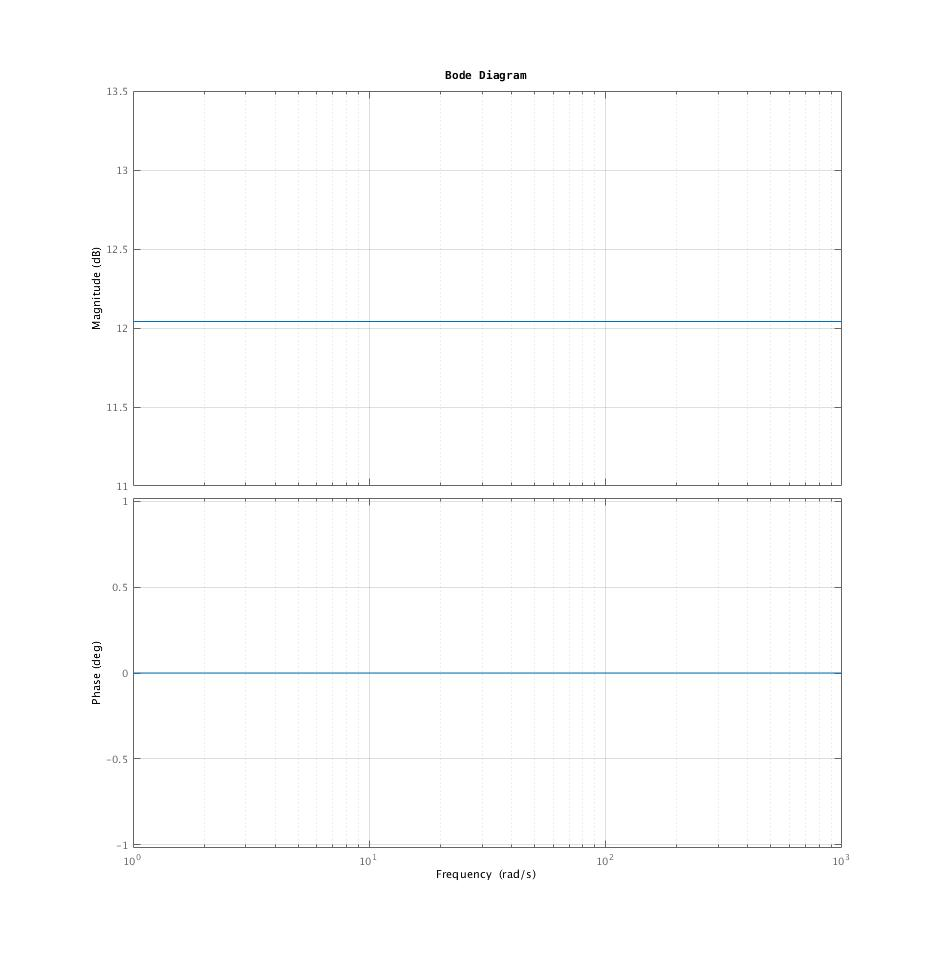
\includegraphics[scale=0.4]{./pictures/termine_guadagno.jpg}
			\end{figure}

		\newpage
		\subsection{Termine Monomio}
			\[
				\begin{aligned}
					\vert H_b(j\omega) \vert_{dB} &= 20\; log_{10}\vert H_b(j\omega) \vert \\
					&= 20\; log_{10}\Big\vert {1\over{j\omega}} \Big\vert \\
					&= -20\; log_{10}\vert j\omega \vert \\
					&= -20\; log_{10}\vert \omega \vert
				\end{aligned}
			\]
			Il che vuol dire che la retta perde \textit{20 dB} per decade in maniera costante. Se avessimo avuto $ g>1 $ ci saremmo trovati nella seguente situazione
			\[
				\begin{aligned}
					\vert H_b(j\omega) \vert_{dB} &= 20\; log_{10}\Big\vert {1\over{(j\omega)^g}} \Big\vert \\
					&= -20g\; log_{10}\vert \omega \vert
				\end{aligned}
			\]
			Per quanto riguarda il diagramma della Fase abbiamo
			\[
				\angle(H_b(j\omega)) = \angle\Big( {1\over{j\omega}} \Big) = -90\degree
			\]
			nel caso avessi $ g>1 $
			\[
				\angle(H_b(j\omega)) = \angle\Big( {1\over{(j\omega)^g}} \Big) = -g90\degree
			\]
			Nel seguente grafico prendimo in considerazione
			\[
				H_b(j\omega) = {1\over{s}}
			\]

			\begin{figure}[h!]
				\centering
				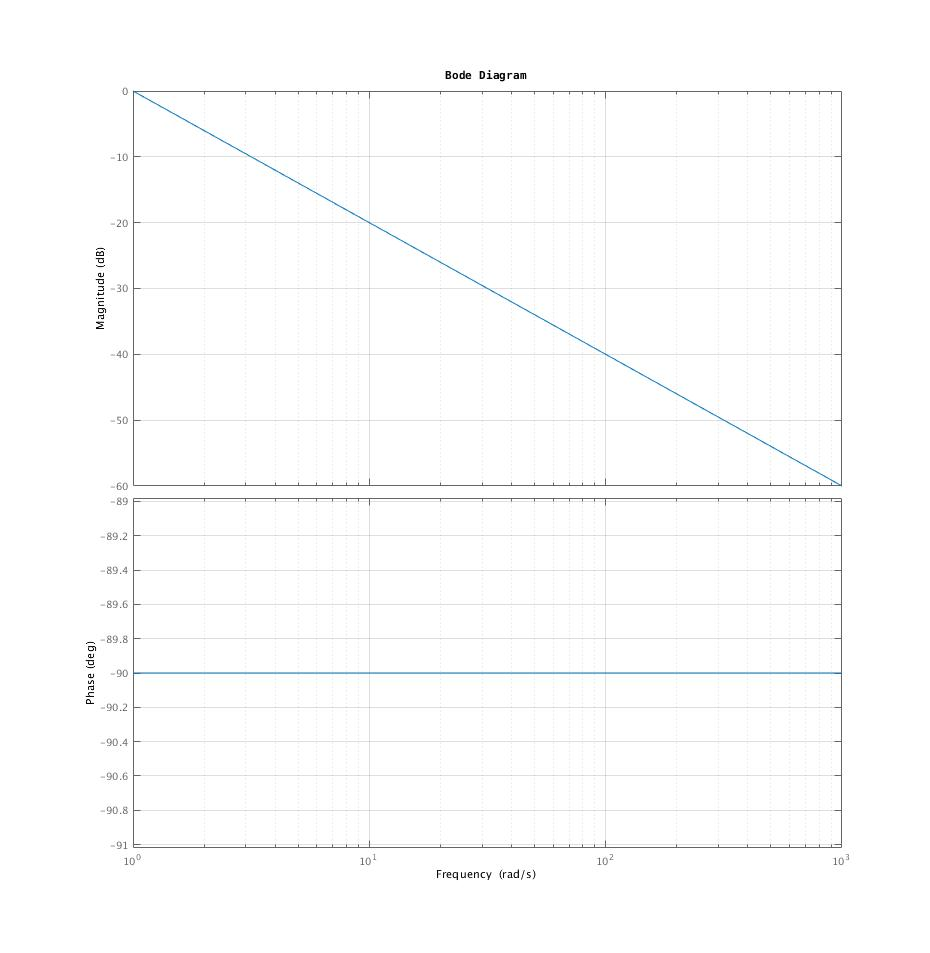
\includegraphics[scale=0.4]{./pictures/termine_monomio.jpg}
			\end{figure}

		\newpage
		\subsection{Termine Binomio}
			In questo caso dobbiamo andare a vedere il comportamento di $ \omega $ quando diventa molto piccolo o molto grande. Procediamo come segue
			\[
				\begin{aligned}
					\vert H_c(j\omega) \vert_{dB} &= 20\; log_{10}\vert H_c(j\omega) \vert \\
					&= 20\; log_{10}\Big\vert {1\over{1 + j\omega\tau}} \Big\vert \\
					&= -20\; log_{10}\vert 1 + j\omega\tau \vert \\
					&= -20\; log_{10}\sqrt{1 + (\omega\tau)^2} \approx \begin{cases}
						-20\; log_{10}\sqrt{1} = 0,\; \omega << {1\over{\vert\tau\vert}} \\
						-20\; log_{10}\vert \omega\tau \vert,\; \omega >> {1\over{\vert\tau\vert}}
					\end{cases}
				\end{aligned}
			\]
			Quindi, asintoticamente, so che avrò \textit{0 dB} fino a $ {0.1\over{\vert\tau\vert}} $ e da $ {10\over{\vert\tau\vert}} $ in poi avrò una perdita costante di \textit{-20 dB} per decade. \\
			Quindi procedo a calcolare il valore in dB in $ \omega = {1\over{\vert\tau\vert}} $
			\[
				\begin{aligned}
					\vert H_c(j{1\over{\vert\tau\vert}}) \vert_{dB} &= 20\; log_{10}\Bigg\vert \underbrace{{1\over{j{1\over{\vert\tau\vert}}\tau}}}_{={1\over{2}}} \Bigg\vert \\
					&= -20\; log_{10}\sqrt{2} \approx -3
				\end{aligned}
			\]
			Se ho $ g>1 $, come nei casi precedenti, moltiplico sia i \textit{-3 dB} che i \textit{-20 dB} per $ g $. Ponendo $ g=2 $ avrei \textit{-40 dB} per decade da $ {10\over{\vert\tau\vert}} $ in poi e passo per \textit{-6 dB} in $ \omega = {1\over{\vert\tau\vert}} $. \\
			Stessa considerazione va fatta per il diagramma della \textit{Fase}, siamo a 0\textdegree fino a $ {0.1\over{\vert\tau\vert}} $ e andiamo a $ \pm90\degree $ in base alla positività o negatività di $ \tau $. In $ \omega = {1\over{\vert\tau\vert}} $ si passa per i $ \pm45\degree $ sempre in base al valore di $ \tau $.
			\\
			Nel seguente grafico prendiamo in considerazione
			\[
				H_c(j\omega) = {1\over{1 + s}}
			\]

			\begin{figure}[h!]
				\centering
				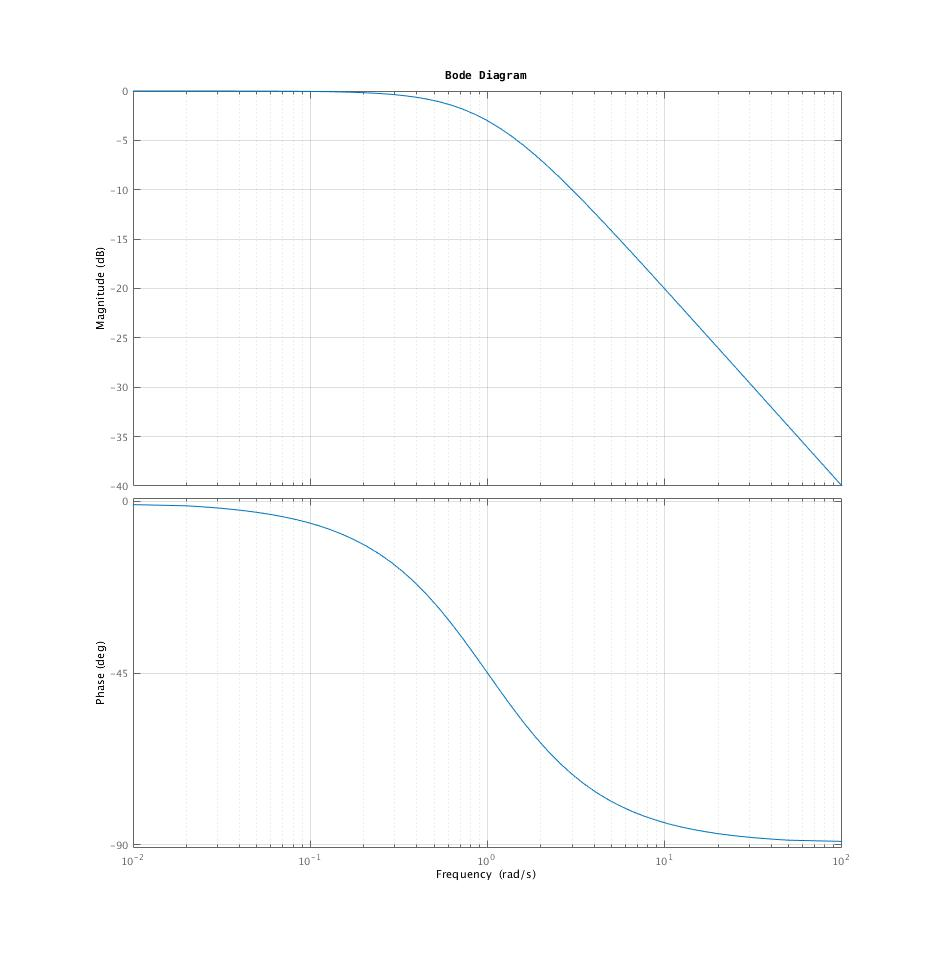
\includegraphics[scale=0.4]{./pictures/termine_binomio.jpg}
			\end{figure}

		\newpage
		\subsection{Termine Trinomio}
			Anche in questo caso, come nel precedente, il grafico dipende dal valore di $ \omega $, questa volta rapportato ad $ \omega_n $.
			\[
				\begin{aligned}
					\vert H_d(j\omega) \vert_{dB} &= 20\; log_{10}\Bigg\vert {1\over{1 - {\omega^2\over{\omega_n^2}} + j{{2\rho\omega}\over{\omega_n}} }} \Bigg\vert \\
					&= -20\; log_{10}\sqrt{(1 + {\omega^2\over{\omega_n^2}})^2 + {{4\rho^2\omega^2\over{\omega_n^2}}}} \\
					&\approx \begin{cases}
						-20\; log_{10}\sqrt{1} \approx 0,\; \omega << \omega_n \\
						-40\; log_{10}{\omega\over{\omega_n}},\; \omega >> \omega_n
					\end{cases}
				\end{aligned}
			\]
			Analogamente a prima ci troviamo, asintoticamnete, a \textit{0 dB} fino a $ 0.1\omega_n $ e da $ 10\omega_n $ avrei una perdita costante di \textit{-40 dB} per decade. \\
			Per il calcolo del valore in \textit{dB} in $ \omega_n $ dipendo da $ \rho $, se $ \rho \to 1 $ tutto il termine trinomio tende ad un \textit{termine binomio elevato al quadrato}. \\
			Un caso limite è quello per $ \vert \rho \vert = 1 $ in cui ho il passaggio per \textit{-6 dB} in $ \omega_n $. \\
			Se $ \vert \rho \vert < 1 $, si può dimostrare che per $ \rho < {1\over{\sqrt{2}}} \approx 0.707 $ ho un massimo detto \textit{Picco di Risonanza} a frequenza $ \omega_R $, detta \textit{Frequenza di Risonanza}
			\[
				\omega_R = \omega_n \sqrt{1 - 2\rho^2}
			\]
			Definisco $ M_R $ \textit{Picco di Risonanza}
			\[
				M_R = \vert H(j\omega_R) \vert = {1\over{2\vert \rho \vert \sqrt{1 - 2\rho^2}}}
			\]
			\textbf{N.B:} Anche questo va portato in dB!\\
			Cerco anche il punto di passaggio per $ \omega_n $
			\[
				\vert H(j\omega_n) \vert = {1\over{2\vert \rho \vert}}
			\]
			Si può notare che più $ \rho $ diventa piccolo, più $ \omega_R $ si sposta verso $ \omega_n $ e, di conseguenza, $ M_R $ è sempre più alto di quota. \\
			Un altro caso limite è per $ \rho = 0 $, ossia $ \omega_R = \omega_n $, in questo caso ho $ M_R \to \infty $ ed ho un asintoto vericale in $ \omega_n $ \\
			Come nel termine binomio, se ho $ g>1 $ da $ 10\omega_n $ in poi avrò una perdita costante di \textit{-40g dB} per decade. \\
			Per quanto riguarda il diagramma della \textit{Fase}, analogamente al termine binomio, rimango a 0\textdegree fino ad $ 0.1\omega_n $ e varrà $ \pm180\degree $ da $ 10\omega_n $ in poi, passo per $ \pm90\degree $ in $ \omega_n $. \\
			Per $ \rho = 0 $ il diagramma della fase coincide con il \textit{Gradino}. \\
			\\
			Nel caso in esempio prendo
			\[
				H_d(j\omega) = {1\over{1 + {1\over{16}}s + {1\over{16}}s^2}}
			\]

			\begin{figure}[h!]
				\centering
				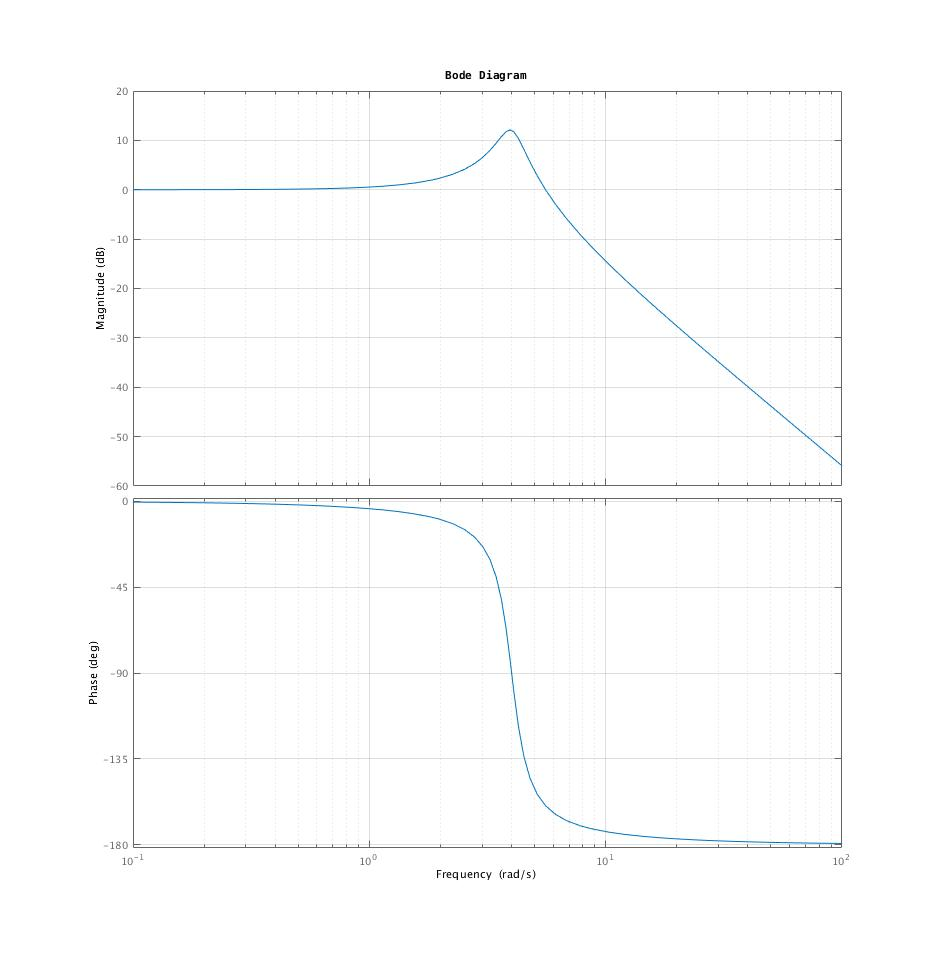
\includegraphics[scale=0.4]{./pictures/termine_trinomio.jpg}
			\end{figure}
			\newpage

	\newpage
	\section{Analisi in $ \Ztransf $}
		\subsection{Trasformata Zeta}
			Equivalente della \textit{Trasformata di Laplace} per il discreto. \\
			Definiamo la \textit{Trasforamta Zeta bilatera} come
			\[
				V(z) = \mathcal{Z}_b[v[n]] = \sum_{k = -\infty}^{+\infty} {v[k]z^{-k}}
			\]
			con $ z = \sigma + j\omega $ variabile complessa. \\
			Considerando solo \textit{sistemi causali}, come per la Trasformata di Laplace, possiamo ridurre gli estremi della sommatoria ottenendo la \textit{Trasformata Zeta unilatera}
			\[
				V(z) = \Ztransf[v[n]] = \sum_{k = 0}^{+\infty} {v[k]z^{-k}}
			\] \\
			Si ricorda che viene utilizzata la notazione con parentesi quadre per indicare un segnale discreto invece di un segnale continuo.

		\subsection{Proprietà della Trasformata Zeta}
			\begin{itemize}
				\item \underline{\textbf{Linearità}} \\
					  \\
					  Dati due segnali discreti generici $ v_1[n] \text{ e } v_2[n] $
					  \[
					  	\Ztransf[av_1[n] + bv_2[n]] = aV_1(z) + bV_2(z)
					  \]
					  \underline{\textit{Dimostrazione:}} \\
					  \[
					  	\begin{aligned}
					  		\Ztransf[av_1[n] + bv_2[n]] &= \sum_{k=0}^{+\infty} {(av_1[k] + bv_2[k])z^{-k}} \\
							&= a \sum_{k=0}^{+\infty} {v_1[k]z^{-k}} + b \sum_{k=0}^{+\infty} {v_2[k]z^{-k}} \\
							&= aV_1(z) + bV_2(z)
					  	\end{aligned}
					  \]
				\item \underline{\textbf{Time Shifting}} \\
					  \\
					  Dato un segnale discreto generico $ v[n] $
					  \[
					  	\Ztransf[v[n - n_0]] = z^{-n_0}V(z)
					  \]
					  \underline{\textit{Dimostrazione:}} \\
					  \[
					  	\begin{aligned}
					  		\Ztransf[v[n - n_0]] &= \sum_{k=0}^{+\infty} {v[k - n_0]z^{-k}} \\
							&= \sum_{j=-n_0}^{+\infty} {v[j]z^{-(j+n_0)}}\;\;\;\;\; (\text{Ponendo } j=k - n_0) \\
							&= \sum_{j=-n_0}^{+\infty} {v[j]z^{-j}z^{-n_0}} \\
							&= z^{-n_0} \sum_{j=-n_0}^{+\infty} {v[j]z^{-j}} \\
							&= z^{-n_0} \sum_{j=0}^{+\infty} {v[j]z^{-j}}
					  	\end{aligned}
					  \]
					  Essendo $ v[n] = 0 $ se $ n<0 $, si ottiene
					  \[
					  	z^{-n_0} \sum_{j=0}^{+\infty} {v[j]z^{-j}} = z^{-n_0}V(z)
					  \]
				\item \underline{\textbf{Moltiplicazione per $ n $ (Differenziazione)}} \\
					  \\
					  Dato un segnale discreto generico $ v[n] $
					  \[
					  	\Ztransf[n\cdot v[n]] = -z V'(z)
					  \]
					  \underline{\textit{Dimostrazione:}} \\
					  Utiliziamo la \textit{Trasformata Zeta bilatera} per la dimostrazione
					  \[
					  	\begin{aligned}
					  		\mathcal{Z}_b[n\cdot v[n]] &= \sum_{k=-\infty}^{+\infty} {n\cdot v[k] z^{-k}} \\
							&= z \sum_{k=-\infty}^{+\infty} {k\cdot v[k] z^{-k - 1}} \\
							&= -z \sum_{k=-\infty}^{+\infty} {v[k] (-kz^{-k - 1})} \\
							&= -z \sum_{k=-\infty}^{+\infty} {v[k] {{d}\over{dz}}(z^{-k})} \\
							&= -z V'(z)
					  	\end{aligned}
					  \]
				\newpage
				\item \underline{\textbf{Moltiplicazione per $ \lambda^n $}} \\
					  \\
					  Dato un segnale discreto generico $ v[n] $
					  \[
					  	\Ztransf[\lambda^n \cdot v[n]] = V\Big( {{z}\over{\lambda}} \Big)
					  \]
					  \underline{\textit{Dimostrazione:}} \\
					  \[
					  	\begin{aligned}
							\Ztransf[\lambda^n \cdot v[n]] &= \sum_{k=0}^{+\infty} {\lambda^k \cdot v[k] z^{-k}} \\
							&= \sum_{k=0}^{+\infty} {v[k] \Big( {{z}\over{\lambda}} \Big)^{-k}} \\
					  		&= V\Big( {{z}\over{\lambda}} \Big)
					  	\end{aligned}
					  \]
				\item \underline{\textbf{Convoluzione}} \\
					  \\
					  Dati due segnali discreti generici $ v_1[n] \text{ e } v_2[n] $
					  \[
					  	\Ztransf[v_1[n] \circledast v_2[n]] = V_1(z)\cdot V_2(z)
					  \]
					  \underline{\textit{Dimostrazione:}} \\
					  Utiliziamo la \textit{Trasformata Zeta bilatera} per la dimostrazione
					  \[
					  	\begin{aligned}
					  		\Ztransf[v_1[n] \circledast v_2[n]] &= \mathcal{Z}_b\Bigg[ \sum_{l=-\infty}^{+\infty} {v_1[l]v_2[n-l]} \Bigg] \\
							&= \sum_{k=-\infty}^{+\infty}\Bigg[ \sum_{l=-\infty}^{+\infty} {v_1[l]v_2[k-l]} \Bigg]z^{-k} \\
							&= \sum_{l=-\infty}^{+\infty} {v_1(l) \Bigg(\sum_{k=-\infty}^{+\infty} {v_2[k-l] z^{-k}}\Bigg)} \\
							&= \Bigg[ \sum_{l=-\infty}^{+\infty} {v_1[l]z^{-l}} \Bigg] \Bigg[ \sum_{k=-\infty}^{+\infty} {v_1[k]z^{-k}} \Bigg] \\
							&= V_1(z)\cdot V_2(z)
					  	\end{aligned}
					  \]
			\end{itemize}

		\subsection{Trasformate Zeta Notevoli}
			\begin{itemize}
				\item \underline{\textbf{Costante}} \\
					  \[
					  	\begin{aligned}
					  		\Ztransf[A] &= \sum_{K=0}^{+\infty} {A\cdot z^{-k}} \\
							&= A \cdot \sum_{K=0}^{+\infty} {z^{-k}} \\
							&= A \cdot {{1}\over{1 - z^{-1}}} \\
							&= A \cdot {{z}\over{z - 1}}
					  	\end{aligned}
					  \]
				\item \underline{\textbf{Impulso}} \\
					  \[
					  	\begin{aligned}
					  		\Ztransf[\delta[n]] &= \sum_{k=0}^{+\infty} {\delta[k] z^{-k}} \\
							&= z^0 = 1
					  	\end{aligned}
					  \]
				\item \underline{\textbf{Impulso traslato}} \\
					  \[
					  	\begin{aligned}
					  		\Ztransf[\delta[n - n_0]] &= \sum_{k=0}^{+\infty} {\delta[k-n_0]z^{-k}} \\
							&= z^{-n_0}
					  	\end{aligned}
					  \]
				\item \underline{\textbf{Gradino}} \\
					  \[
					  	\begin{aligned}
							\Ztransf[\delta_{-1}[n]] &= \sum_{k=0}^{+\infty} {\delta_{-1}[n] z^{-k}} \\
							&= \sum_{k=0}^{+\infty} {z^{-k}} \\
							&= {{1}\over{1 - z^{-1}}} = {{z}\over{z - 1}}
					  	\end{aligned}
					  \]
				\item \underline{\textbf{Esponenziale}} \\
					  \\
					  Consideriamo un esponenziale generico $ \lambda^n $ moltiplicato per un gradino $ \delta_{-1}[n] $
					  \[
					  	\begin{aligned}
							\Ztransf[\lambda^n\delta_{-1}[n]] &= \Ztransf[\delta_{-1}[n]] \cdot \Big( {{z}\over{\lambda}} \Big) \\
							&= {{{{z}\over{\lambda}}}\over{{{z}\over{\lambda}} - 1}} \\
					  		&= {{z}\over{z - \lambda}}
					  	\end{aligned}
					  \]
				\item \underline{\textbf{Segnale Sinusoidale}} \\
					  \\
					  Consideriamo il segnale sinusoidale $ v[n] = cos(\theta n + \phi) $ moltiplicato per un gradino $ \delta_{-1}[n] $. \\
					  Si ricordi che la \textit{Formula di Eulero} è valida anche per i segnali discreti.
					  \[
					  	\begin{aligned}
					  		\Ztransf[cos(\theta n + \phi)\delta_{-1}[n]] &= \Ztransf\Big[{{e^{j(\theta n + \phi)} + e^{-j(\theta n + \phi)}}\over{2}}\delta_{-1}[n]\Big] \\
							&= {{1}\over{2}} \Big( e^{j\phi} \Ztransf[(e^{j\theta})^k \delta_{-1}[k]] + e^{-j\phi} \Ztransf[(e^{-j\theta})^k \delta_{-1}[k]] \Big) \\
							&= {{1}\over{2}} \Big( {{ze^{j\theta}}\over{z - e^{j\theta}}} + {{ze^{-j\phi}}\over{z - e^{-j\phi}}} \Big) \\
							&= {{1}\over{2}} \Big( {{z^2 e^{j\phi} - ze^{j(\phi - \theta)} + z^2e^{-j\phi} - ze^{-j(\phi - \theta)}}\over{z^2 - ze^{j\theta} - ze^{-j\theta} + 1}} \Big) \\
							&= {{z(cos(\phi)z - cos(\phi - 	\theta))}\over{z^2 -2cos(\theta)z + 1}}
					  	\end{aligned}
					  \]
			\end{itemize}

		\subsection{Antitrasformata Zeta}
			Per tornare dal \textit{dominio complesso} al \textit{dominio del tempo}, analoga all'\textit{Antitarsformata di Laplace} per i segnali continui.
			\[
				\AntiZtransf[V(z)] = v[n]
			\]
			Il calcolo della \textit{risposta del sistema} è identico a quello usato con la Trasormata di Laplace, applicato però a segnali discreti.
			\[
				\begin{aligned}
					V(z) &= V_l(z) + V_f(z) \\
					&= {{p(z)}\over{d(z)}} + H(z)U(z) \\
					&= {{p(z)}\over{d(z)}} + {{n(z)}\over{d(z)}}U(z)
				\end{aligned}
			\]
			Per trovare $ V(z) $ ci si può avvalere della forma utilizzata con la \textit{Trasforamta di Laplace}, facendo attenzione al numeratore $ z $.
			\[
				\begin{aligned}
					V(z) &= {{n(z)}\over{\prod_{i=1}^{r'} {(z - \lambda'_{i})^{\mu'_i}}}} \\
					&= \sum_{i=1}^{r'} {\sum_{l=1}^{\mu'_i} {C_{i,l} {{z}\over{(z - \lambda'_{i})^{l}}}}} = V'(s)
				\end{aligned}
			\]
			I vari $ C_{i,l} $ si ottengono con il metodo dei fratti semplici
			\[
				C_{i,l} = {{d^{{\mu'_i}-l}}\over{dz^{{\mu'_i}-l}}} \Bigg( (z - \lambda'_{i})^{\mu'_i} {{V'(z)}\over{z}} \Bigg) \Bigg\vert_{z=\lambda'_i}
			\]

	\section{Esercizi}
		\subsection{Risposta di un Sistema}
			Calcolare la risposta di un sistema espresso nella forma di un \textit{Problema di Cauchy}.
			\[
				\begin{cases}
					v''(t) - 5v'(t) + 4v(t) = u'(t) - 3u(t) \\
					v(0) = 0 \\
					v'(0) = 1
				\end{cases}
			\]
			con
			\[
				u(t) = e^t \delta_{-1}(t)
			\]
			\begin{enumerate}
				\item Risolvo l'equazione caratteristica per trovare l'\textit{Evoluzione Libera} \\
					  \[
					  	\begin{gathered}
					  		s^2 - 5s + 4 = 0\quad\quad \Delta = 9 \\
							\\
							\lambda_{1,2} = {{5 \pm \sqrt{9}}\over{2}} = 4 \text{ e } 1
					  	\end{gathered}
					  \]
					  Ottengo quindi l'Evoluzione Libera, indicata da $ v_l(t) $
					  \[
					  	\begin{gathered}
					  		v_l(t) = C_1e^{4t} + C_2e^t \\
							v'_l(t) = 4C_1e^{4t} + C_2e^t
					  	\end{gathered}
					  \]
				\item Metto a sistema ed impongo le condizioni inizali
					  \[
						\begin{cases}
						  	C_1 + C_2 = 0\; \rightarrow\; C_1 = -C_2\; \rightarrow\; C_1 = {{1}\over{3}} \\
							4C_1 + C_2 = 1\; \rightarrow\; -3C_2 = 1\; \rightarrow\; C_2 = -{{1}\over{3}}
						\end{cases}
					  \]
					  Ottengo quindi la \textit{Risposta Libera}
					  \[
					  	v_l(t) = {{1}\over{3}}e^{4t} - {{1}\over{3}}e^{t}
					  \]
				\item Calcolo l'\textit{Evoluzione Forzata}
					  \[
					  	\begin{gathered}
							h(t) = (d_1e^{4t} + d_2e^t)\delta_{-1}(t) \\
							h'(t) = (4d_1e^{4t} + d_2e^t)\delta_{-1}(t) + (d_1e^{4t} + d_2e^t)\delta(t) \\
							h''(t) = (16d_1e^{4t} + d_2e^t)\delta_{-1}(t) + 2(4d_1e^{4t} + d_2e^t)\delta(t) + (d_1e^{4t} + d_2e^t)\delta'(t)
					  	\end{gathered}
					  \]
					  E sostituisco all'equazione del sistema nella seguente forma
					  \[
					  	h''(t) - 5h'(t) + 4h(t) = \delta'(t) - 3\delta(t)
					  \]
					  \[
					  	\begin{aligned}
					  		&(16d_1e^{4t} + d_2e^t)\delta_{-1}(t) + 2(4d_1e^{4t} + d_2e^t)\delta(t) + (d_1e^{4t} + d_2e^t)\delta'(t) + \\
							&\quad -5((4d_1e^{4t} + d_2e^t)\delta_{-1}(t) + (d_1e^{4t} + d_2e^t)\delta(t)) + 4((d_1e^{4t} + d_2e^t)\delta_{-1}(t)) \\
							&\quad = \delta'(t) - 3\delta(t) \\
							\\
							&=(16d_1e^{4t} + d_2e^t)\delta_{-1}(t) + (8d_1e^{4t} + 2d_2e^t)\delta(t) + (d_1e^{4t} + d_2e^t)\delta'(t) + \\
							&\quad - (20d_1e^{4t} + 5d_2e^t)\delta_{-1}(t) - (5d_1e^{4t} +5d_2e^t)\delta(t) + (4d_1e^{4t} + 4d_2e^t)\delta_{-1}(t) + \\
							&\quad - \delta'(t) + 3\delta(t) = 0
					  	\end{aligned}
					  \]
					  Raccolgo e metto a sistema
					  \[
					  	\begin{aligned}
							&\begin{cases}
								\delta_{-1}(t)((\cancel{16d_1} + \cancel{d_2}) - (\cancel{20d_1} + \cancel{5d_2}) + (\cancel{4d_1} + \cancel{4d_2})) = 0 \\
								\delta(t)((8d_1 + 2d_2) - (5d_1 + 5d_2) + 3) = 0 \\
								\delta'(t)((d_1 + d_2) - 1) = 0
							\end{cases} \\
							\\
					  		&= \begin{cases}
								3d_1 - 3d_2 + 3 = 0\; \rightarrow\; 3(-d_2 + 1) - 3d_2 + 3 = 0 \\
								d_1 + d_2 - 1 = 0\; \rightarrow\; d_1 = -d_2 + 1
							\end{cases} \\
							\\
							&= \begin{cases}
								-3d_2 +3 -3d_2 + 3 = 0\; \rightarrow\; -6d_2 = -6\; \rightarrow\; d_2 = 1 \\
								d_1 = -1 + 1\; \rightarrow\; d_1 = 0
							\end{cases}
					  	\end{aligned}
					  \]
					  Ottengo quindi l'Evoluzione Forzata, scrivendola con la notazione $ h(t) $
					  \[
					  	h(t) = e^t\delta_{-1}(t)
					  \]
				\item Calcolo la \textit{Risposta Forzata}
					  \[
					  	\begin{aligned}
					  		v_f(t) &= \int_{0}^{t} {(e^{\tau}\underbrace{\delta_{-1}(\tau)}_{=1})(e^{(t-\tau)}\underbrace{\delta_{-1}(t-\tau)}_{=1})\; d\tau} \\
							&= e^t \Bigg( \int_{0}^{t} {e^0\; d\tau} \Bigg) \delta_{-1}(t) \\
							&= {{1}\over{2}}e^t (t-0) \delta_{-1}(t) \\
							&= {{1}\over{2}}e^t t \delta_{-1}(t)
					  	\end{aligned}
					  \]
				\item Sommo Risposta Libera e Risposta Forzata per ottenere la \textit{Risposta Totale}
					  \[
					  	\begin{aligned}
							v(t) &= v_l(t) + v_f(t) \\
					  		&= {{1}\over{3}}e^{4t} - {{1}\over{3}}e^t + {{1}\over{2}}e^t t \delta_{-1}(t)
					  	\end{aligned}
					  \]
			\end{enumerate}

		\newpage
		\subsection{Stabilità Asintotica e BIBO Stabilità}
		\[
			\begin{cases}
				v''(t) + v'(t) - 2v(t) = u'(t) - u(t) \\
				v'(0) = 0 \\
				v(0) = 3 \\
				u(t) = e^{-2t}\delta_{-1}(t)
			\end{cases}
		\]
		\begin{enumerate}
			\item Controllo le radici del polinomio caratteristico ricordando che devono entrambe essere $ <0 $ per avere \textit{Stabilità asintotica}
			\[
				\begin{gathered}
					s^2 + s - 2 = 0 \\
					\Delta = 1 + 8 = 9 \\
					\\
					\lambda_{1,2} = {{1 \pm 3}\over{2}} = 2 \text{ e } -1
				\end{gathered}
			\]
			Quindi \textbf{non} ho stabilità asintotica.
			\item Nel caso al punto \textit{1} risultasse stabilità asintotica avremo anche \textit{BIBO Stabilità}, in quanto \textbf{Stabilità Asintotica $ \Rightarrow $ BIBO Stabilità}. \\
			In caso contrario analizaimo $ H(s) $ per il sistema in questione, ricordando che
			\[
				H(s) = {{Eq.\;\; Caratteristica\;\; 2^{\circ}\;\; Membro}\over{Eq.\;\; Caratteristica\;\; 1^{\circ}\;\; Membro}}
			\]
			nel nostro caso
			\[
				H(s) = {{s - 1}\over{(s - 2)(s + 1)}}
			\]
			Risolvo quindi con il \textit{Metodo dei Fratti Semplici}
			\[
				H(s) = {{s - 1}\over{(s - 2)(s + 1)}} = A{{1}\over{s - 2}} + B{{1}\over{s + 1}}
			\]
			\\
			\[
				A = (s + 1)H(s)\vert_{s=-1} = {{s - 1}\over{s - 2}}\Big\vert_{s=-1} = {{2}\over{3}}
			\]
			\\
			\[
				B = (s - 2)H(s)\vert_{s=2} = {{s - 1}\over{s + 1}}\Big\vert_{s=2} = {{1}\over{3}}
			\]
			Quindi riscrivo $ H(s) $ nella forma
			\[
				{{2}\over{3}}\Bigg( {{1}\over{s + 1}} \Bigg) + {{1}\over{3}}\Bigg( {{1}\over{s - 2}} \Bigg)
			\]
			Passaimo ora nel \textit{dominio del tempo} tramite l'\textit{Antitrasforamta di Laplace}
			\[
				h(t) = \AntiLaplace[H(s)] = {{2}\over{3}}e^{-t} + {{1}\over{3}}e^{2t}
			\]
			Se ne deduce che il sistema non è nemmeno \textit{BIBO Stabile} in quanto le $ \lambda $ sono positive.
		\end{enumerate}

		\newpage
		\subsection{Risposta di un Sistema tramite Trasf. di Laplace}
			Calcolare la risposta di un sistema espresso nella forma di un \textit{Problema di Cauchy} utilizzando la \textit{Trasforamta di Laplace}.
			\[
				\begin{cases}
					v''(t) - 5v'(t) + 4v(t) = u'(t) - 3u(t) \\
					v(0) = 0 \\
					v'(0) = 1
				\end{cases}
			\]
			con
			\[
				u(t) = e^t \delta_{-1}(t)
			\]
			\begin{enumerate}
				\item Trasformo il sistema tramite \textit{Trasforamta di Laplace}
					  \[
					  	\begin{gathered}
							\Laplace[v''(t) - 5v'(t) + 4v(t) = u'(t) - 3u(t)] \\
							\downarrow \\
					  		(s^2V(s) - sv(0) - v'(0)) - 5(sV(s) - v(0)) + 4(V(s)) = (sU(s) - v(0)) - 3(U(s))
					  	\end{gathered}
					  \]
					  Imponendo le condizioni iniziali otteniamo
					  \[
					  	s^2V(s) - 1 - 5sV(s) + 4V(s) = sU(s) -3U(s)
					  \]
					  Raccolgo
					  \[
					  	V(s)(\underbrace{s^2 - 5s + 4}_{(s - 1)(s - 4)}) = 1 + (s - 3)U(s)
					  \]
					  che equivale a
					  \[
					  	V(s) = {{1}\over{(s - 1)(s - 4)}} + {{(s - 3)}\over{(s - 1)(s - 4)}}U(s)
					  \]
					  dove
					  \begin{itemize}
					  	\item $ {{1}\over{(s - 1)(s - 4)}} = V_l(s) $
						\item $ {{(s - 3)}\over{(s - 1)(s - 4)}} = H(s) $
						\item $ U(s) = \Laplace[u(t)] = {{1}\over{s - 1}} $
					  \end{itemize}
					  Riscrivendo tutto come un unica frazione
					  \[
					  	\begin{aligned}
							V(s) &= {{1}\over{(s - 1)(s - 4)}} + {{(s - 3)}\over{(s - 1)^2(s - 4)}} \\
					  		&= {{2(s - 2)}\over{(s - 1)^2(s - 4)}} = F(s) \\
					  	\end{aligned}
					  \]
				\item Risolvo utilizzando il Metodo dei Fratti Semplici
				 	  \[
					  	V(s) = {{A}\over{(s - 4)}} + {{B}\over{(s - 1)}} + {{C}\over{(s - 1)^2}}
					  \]
					  \[
					  	\begin{aligned}
					  		A &= (s - 4)F(s)\vert_{s=4} \\
							&= \cancel{(s - 4)}{{2(s - 2)}\over{(s - 1)^2\cancel{(s - 4)}}}\Bigg\vert_{s=4} \\
							&= {{2(s - 2)}\over{(s - 1)^2}}\Big\vert_{s=4} = {{4}\over{9}}
					  	\end{aligned}
					  \]
					  \\
					  \[
					  	\begin{aligned}
							B &= ((s - 1)^2 F(s))'\vert_{s=1} \\
							&= 2\Bigg( \cancel{(s - 1)^2}{{(s - 2)}\over{\cancel{(s-1)^2}(s - 4)}} \Bigg)'\Bigg\vert_{s=1} \\
							&= 2\Bigg( {{s - 2}\over{s - 4}} \Bigg)'\Bigg\vert_{s=1} \\
							&= {{-4}\over{(s - 4)^2}}\Bigg\vert_{s=1} = -{{4}\over{9}}
					  	\end{aligned}
					  \]
					  \\
					  \[
						\begin{aligned}
							C &= (s - 1)^2 F(s)\vert_{s=1} \\
							&= 2\Bigg( {{s - 2}\over{s - 4}} \Bigg)\Bigg\vert_{s=1} \\
							&= {{2s - 4}\over{s - 4}}\Bigg\vert_{s=1} = {{2}\over{3}}
						\end{aligned}
					  \]
					  ed ottengo la \textit{Risposta Totale} nel Dominio Complesso
					  \[
					  	V(s) = {{4}\over{9}}\Bigg( {{1}\over{s - 4}} \Bigg) - {{4}\over{9}}\Bigg( {{1}\over{s - 1}} \Bigg) + {{2}\over{3}}\Bigg( {{1}\over{(s - 1)^2}} \Bigg)
					  \]
				\item Applico l'\textit{Antitrasformata di Laplace} alla Risposta Toatale
					  \[
					  	\begin{aligned}
							v(t) &= \AntiLaplace[V(s)] \\
					  		&= \Bigg( {{4}\over{9}}e^{4t} - {{4}\over{9}}e^t + {{2}\over{3}}te^t \Bigg)\delta_{-1}(t)
					  	\end{aligned}
					  \]
			\end{enumerate}

		\newpage
		\subsection{Risposta di un Sistema Discreto}
			\[
				\begin{cases}
					v[n]-v[n-2]=u[n-1]+2u[n-2] \\
					v[-1] = 1 \\
					v[n-2] = -2
				\end{cases}
			\]
			\begin{enumerate}
				\item Risolvo l'equazione caratterisctica
					  \[
					  	\begin{gathered}
					  		z^2 - 1 = 0 \\
							\Delta = 0 + 4 = 4 \\
							\\
							\lambda_{1,2} = {{0 \pm 2}\over{2}} = 1 \text{ e } -1
 					  	\end{gathered}
					  \]
					  e trovo l'Evoluzione Libera
					  \[
					  	v_l[n] = C_1(1)^n + C_2(-1)^n
					  \]
				\item Imposto il sistema con le condizioni iniziali
					  \[
					  	\begin{gathered}
							\begin{cases}
								C_1 - C_2 = 1 \\
								C_1 + C_2 = -2\; \rightarrow\; 2C_2 = -3\; \rightarrow\; C_2 = -{{3}\over{2}}
							\end{cases} \\
					  		\begin{cases}
					  			C_1 = -{{3}\over{2}} + 1\; \rightarrow\; C_1 = -{{1}\over{2}} \\
								C_2 = -{{3}\over{2}}
					  		\end{cases}
					  	\end{gathered}
					  \]
					  e trovo la \textit{Risposta Libera}
					  \[
					  	v_l[n] = -{{1}\over{2}}(1)^n - {{3}\over{2}}(-1)^n
					  \]
				\item Cerco Risposta Impulsiva
					  \[
					  	h[n] - h[n - 2] = \delta[n - 1] + 2\delta[n - 2]
					  \]
					  Risolvendo nella forma
					  \[
					  	h[n] = d_0\delta[n] + (d_1(1)^n + d_2(-1)^n)\delta_{-1}[n - 1]
					  \]
					  Calcolo gli $ h[n] $ nel sistema per
					  \begin{itemize}
					  	\item \textbf{$ n=0 $}
							  \[
							  	h[0] - \underbrace{\cancel{h[-2]}}_{=0} = \underbrace{\cancel{\delta[-1]}}_{=0} + \underbrace{\cancel{2\delta[-2]}}_{=0}\; \rightarrow\; h[0] = 0
							  \]
						\item \textbf{$ n=1 $}
							  \[
							  	h[1] - \underbrace{\cancel{h[-1]}}_{=0} = \delta[0] + \underbrace{\cancel{2\delta[-1]}}_{=0}\; \rightarrow\; h[1] = 1
							  \]
						\item \textbf{$ n=2 $}
							  \[
							  	h[2] - h[0] = \underbrace{\cancel{\delta[1]}}_{=0} + 2\delta[0]\; \rightarrow\; h[2] = 2
							  \]
					  \end{itemize}
					  Imposto il sistema
					  \[
					  	\begin{cases}
					  		d_0\delta[0] + (d_1(1)^0 + d_2(-1)^0)\underbrace{\delta_{-1}[-1]}_{=0} = 0 \\
							\underbrace{\cancel{d_0\delta[1]}}_{=0} + (d_1(1) + d_2(-1))\underbrace{\delta_{-1}[0]}_{=1} = 1 \\
							\underbrace{\cancel{d_0\delta[2]}}_{=0} + (d_1(1)^2 + d_2(-1)^2)\underbrace{\delta_{-1}[1]}_{=1} = 2
					  	\end{cases}
					  \]
					  \[
					  	\begin{cases}
					  		d_0 = 0 \\
							d_1 - d_2 = 1\; \rightarrow\; d_1 = d_2 + 1\; \rightarrow\; d_1 = {{3}\over{2}} \\
							d_1 + d_2 = 2\; \rightarrow\; 2d_2 = 1\; \rightarrow\; d_2 = {{1}\over{2}}
					  	\end{cases}
					  \]
					  Quindi
					  \[
					  	h[n] = ({{3}\over{2}}(1)^n + {{1}\over{2}}(-1)^n)\delta_{-1}[n - 1]
					  \]
				\item Cerco \textit{Risposta Forzata}
					  \[
					  	v_f[n] = \sum_{i=0}^{n} {h[i]u[n - i]}
					  \]
				\item \textit{Risposta Totale}
					  \[
					  	\begin{aligned}
							v[n] &= v_l[n] + v_f[n] \\
							&= -{{1}\over{2}}(1)^n - {{3}\over{2}}(-1)^n + \sum_{i=0}^{n} {h[i]u[n - i]}
					  	\end{aligned}
					  \]
			\end{enumerate}

		\newpage
		\subsection{Risposta di un Sistema Discreto con Trasf. Zeta}
			\[
				\begin{cases}
					v[n] - v[n - 2] = u[n - 1] + 2u[n - 2] \\
					v[-1] = 1 \\
					v[-2] = -2 \\
					u[n] = (-1)^n \delta_{-1}[n]
				\end{cases}
			\]
			\begin{enumerate}
				\item Risolvo l'equazione caratteristica
					  \[
					  	\begin{gathered}
					  		z^2 - 1 = 0 \\
							\Delta = 0 + 4 = 4 \\
							\\
							\lambda_{1,2} = {{0 \pm 2}\over{2}} = 1 \text{ e } -1
					  	\end{gathered}
					  \]
				\item Applico \textit{Trasforamta Zeta} al sistema
					  \[
					  	\begin{gathered}
							\Ztransf[v[n] - v[n - 2] = u[n - 1] + 2u[n - 2]] \\
							\downarrow \\
							\begin{aligned}
								&= z^0 V(z) - z^{-2}(V(z) + z^1v[-1] + z^2v[-2]) = z^{-1}(U(z) z^1\underbrace{u[-1]}_{0}) + \\
								&\quad\; + z^{-2}(U(z) + z^1\underbrace{u[-1]}_{0} + z^2\underbrace{u[-2]}_{0}) \\
								\\
								&= z^0V(z) - z^{-2}V(z) - z^{-1} + 2z^0 = z^{-1}U(z) + 2z^{-2}U(z)
 							\end{aligned}
					  	\end{gathered}
					  \]
				\item Moltiplico per $ z^n $, ossia $ z^2 $ perchè ho 2 coefficienti
					  \[
					  	\begin{gathered}
					  		&\begin{aligned}
					  			z^2V(z) - z^0V(z) - z^1 + 2z^2 &= z^1U(z) + 2z^0U(z) \\
					  			(z^2 - 1)V(z) &= -2z^2 + z + (z + 2)U(z)
					  		\end{aligned} \\
					  		\\
					  		& V(z) = {{z(-2z + 1)}\over{(z - 1)(z + 1)}} + {{z + 2}\over{(z - 1)(z + 1)}}U(z)
					  	\end{gathered}
					  \]
					  da cui possiamo capire che
					  \begin{itemize}
					  	\item $ V_l(z) = {{z(-2z + 1)}\over{(z - 1)(z + 1)}} $
						\item $ H(z) = {{z + 2}\over{(z - 1)(z + 1)}} $
						\item $ U(z) = \Ztransf[u[n]] = {{z}\over{z + 1}} $
					  \end{itemize}
					  quindi
					  \[
					  	\begin{aligned}
					  		V(z) &= {{z(-2z + 1)}\over{(z - 1)(z + 1)}} + {{z + 2}\over{(z - 1)(z + 1)}} \cdot {{z}\over{z + 1}} \\
							&= {{z(-2z + 1)}\over{(z - 1)(z + 1)}} + {{z^2 + 2z}\over{(z - 1)(z + 1)^2}} \\
							&= {{z^2 + 2z + (z + 1)(-2z^2 + z)}\over{(z - 1)(z + 1)^2}} \\
							&= {{z(-2z^2 + 3)}\over{(z - 1)(z + 1)^2}} \\
							&= A{{z}\over{z - 1}} + B{{z}\over{z + 1}} + C{{z}\over{(z + 1)^2}}
					  	\end{aligned}
					  \]
				\item Risolvo con il \textit{Metodo dei Fratti Semplici}
					  \[
					  	\begin{aligned}
					  		A &= (z - 1){{V(z)}\over{z}}\Bigg\vert_{z=1} \\
							&= \cancel{(z - 1)}\Bigg( {{-2z^2 + 3}\over{\cancel{(z - 1)}(z + 1)^2}} \Bigg)\Bigg\vert_{z=1} \\
							&= {{-2z^2 + 3}\over{(z + 1)^2}}\Bigg\vert_{z=1} = {{1}\over{4}}
					  	\end{aligned}
					  \]
					  \[
					  	\begin{aligned}
							B &= \Bigg( \cancel{(z + 1)^2}\Bigg( {{-2z^2 + 3}\over{(z - 1)\cancel{(z - 1)^2}}} \Bigg) \Bigg)'\Bigg\vert_{z=-1} \\
							&= {{-4z^2 + 4z + 2z^2 - 3}\over{(z - 1)^2}}\Bigg\vert_{z=-1} \\
					  		&= {{-2z^2 + 4z - 3}\over{(z - 1)^2}}\Bigg\vert_{z=-1} = -{{9}\over{4}}
					  	\end{aligned}
					  \]
					  \[
					  	\begin{aligned}
							C &= \cancel{(z + 1)^2}\Bigg( {{-2z^2 + 3}\over{(z - 1)\cancel{(z + 1)^2}}} \Bigg)\Bigg\vert_{z=-1} \\
							&= {{-2z^2 - 3}\over{z - 1}}\Bigg\vert_{z=-1} \\
					  		&= -{{1}\over{2}}
					  	\end{aligned}
					  \]
					  Quindi
					  \[
					  	V(z) = {{1}\over{4}}\Bigg( {{z}\over{z - 1}} \Bigg) - {{9}\over{4}}\Bigg( {{z}\over{z + 1}} \Bigg) - {{1}\over{2}}\Bigg( {{z}\over{(z + 1)^2}} \Bigg)
					  \]
				\item Applico l'\textit{Antitrasformata Zeta}
					  \[
					  	\begin{aligned}
							v[n] &= \mathcal{Z}^{-1}[V(z)] \\
					  		&= \Bigg( {{1}\over{4}}(1)^n - {{9}\over{4}}(-1)^n - {{1}\over{2}}n(-1)^n \Bigg)\delta_{-1}[n]
					  	\end{aligned}
					  \]
			\end{enumerate}

		\subsection{Metodo di Mason Semplificazione Schemi a Blocchi}
			\begin{figure}[h!]
				\centering
				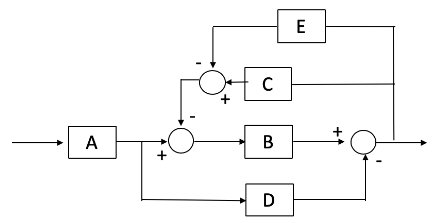
\includegraphics[scale=0.7]{./pictures/diagramma_blocchi.png}
			\end{figure}
			\begin{enumerate}
				\item Cerco tutti i \textit{percorsi} $ P_i $ e tutti i \textit{cicli} $ P_{ij} $ nel grafo
					  \begin{center}
				    	\begin{tabular}{ c c }
					  	  	\toprule
					  	  	$ P_1 = AB  $ & $ P_{11} = -BC $ \\
					  	  	\hline
					  	  	$ P_2 = -AD $ & $ P_{12} = BE $ \\
					  	  	\bottomrule
				    	\end{tabular}
				  	  \end{center}
				\item Calcolo $ \Delta $
					  \[
					  	\Delta = 1 - (BE - BC) = 1 - BE + BC
					  \]
				\item Calcolo la \textit{Funzione di Trasferimento}
					  \[
					  	FdT = {{AB - AD}\over{1 - BE + BC}}
					  \]
			\end{enumerate}

\end{document}
